 \documentclass[12pt]{article}
%\graphicspath{{figures/}}
\usepackage{subfigure}
\usepackage{mathrsfs}
\usepackage{subfigure}
\usepackage{mathrsfs}

\usepackage{amsmath}
\usepackage{graphicx}
\usepackage{subfigure}

\usepackage{mathptmx}
\usepackage{helvet}
\usepackage{multirow}
\usepackage{lineno}
\usepackage{mathrsfs}
\usepackage{rotating}
\usepackage{xspace}
\usepackage{units}

\usepackage{authblk}
\renewcommand\Authands{, } % avoid ``. and'' for last author
\renewcommand\Affilfont{\itshape\small} % affiliation formatting


\def\Wtaunu{\ensuremath{W\to\tau^{\pm}\nu}\xspace}
\def\Htaunu{\ensuremath{H\to\tau^{\pm}\nu}\xspace}
\def\WHtaunu{\ensuremath{W/H\to\tau^{\pm}\nu}\xspace}
\def\ZHtautau{\ensuremath{Z/H\to\tau^{-}\tau^{+}}\xspace}
\def\Ztautau{\ensuremath{Z/\gamma^{*}\to\tau^{-}\tau^{+}}\xspace}
\def\Zee{\ensuremath{Z/\gamma^{*}\to e^{-}e^{+}}\xspace}
\def\Zmm{\ensuremath{Z/\gamma^{*}\to\mu^{-}\mu^{+}}\xspace}
\def\Htautau{\ensuremath{H\to\tau^{-}\tau^{+}}\xspace}
\def\TauNu{\ensuremath{\tau^{\pm}\nu}\xspace}
\def\TauTau{\ensuremath{\tau^{-}\tau^{+}}\xspace}
\def\Tau{\ensuremath{\tau}\xspace}
\def\TauMin{\ensuremath{\tau^-}\xspace}
\def\TauPlus{\ensuremath{\tau^+}\xspace}
\def\RHO{\ensuremath{\pi^{-}\pi^{0}\nu}\xspace}
\def\ARES{\ensuremath{\pi^{-}\pi^{0}\pi^{0}\nu}\xspace}
\def\ARESMULTI{\ensuremath{\pi^{-}\pi^{-}\pi^{+}\nu}\xspace}
\def\PI{\ensuremath{\pi^{-}\nu}\xspace}
\def\KA{\ensuremath{K^{-}\nu}\xspace}
\def\PTAUZ{\ensuremath{P_{\tau}^{\mathrm{Z}}}\xspace}
\def\PTAU{\ensuremath{P_{\tau}}\xspace}
\def\ZGAMMA{\ensuremath{Z/\gamma^{*}}\xspace}



\begin{document}
\begin{titlepage}
\begin{flushright}
{ CERN-PH-TH/20011-307}
\end{flushright}

% Title
\vspace{0.2cm}
\begin{center}
{\Huge \bf {\tt TauSpinner} program for studies on spin effect in $\tau$
  production at the LHC.}
\end{center}

\vspace*{5mm}

\begin{center}
{\bf {Z. Czyczula}$^a$,
{T. Przedzinski}$^b$ and
{Z. Was}$^{c,d}$} \\

{\em $^a$ Yale University, New Haven, USA} \\
{\em $^b$ Institute of Physics, Jagiellonian University, Cracow, Poland} \\
{\em $^c$ Theory Group, Physics Department, CERN, CH-1211, Geneva 23, Switzerland} \\
{\em $^d$ Institute of Nuclear Physics, Cracow, Poland}
\end{center}


\vspace{.1 cm}
\begin{center}
{\bf   ABSTRACT  }
\end{center}
{
Final states involving \Tau leptons are important components of
searches for new pacticles at the Large Hadron Collider (LHC). 
Proper treatment of \Tau spin
effects in the Monte Carlo (MC) simulations is important for
understanding the detector acceptance as well as for 
the measurement of \Tau polarization and \Tau spin correlations.
In this note we present a {\tt TauSpinner} package designed 
to simulate the spin effects. It relies on the information
on the four-momenta of the \Tau leptons and their decay 
products being available in the analyzed data. 
The flavor and the four-momentum of the boson decaying to the \TauTau or
\TauNu pair need to be known. In the $Z/\gamma^*$ case the information on the incoming
quarks is attributed from the intermediate boson
kinematics, and the parton distribution functions (PDF's).
{\tt TauSpinner} is the first algorithm suitable for emulation of \Tau spin effects
in \Tau-embedded samples. It is also the first tool which offers flexibility to a user
to simulate a desired spin effect at the analysis level. An algorithm to attribute $\tau$  helicity states to the previously generated sample is also provided.
}

\vspace{ 1 cm}
%%%%%%%%%%%%%%%%%%%%%%%%%%%%%%%%%%%%
\begin{flushleft}
CERN-PH-TH/2011-307 \\
December 2011
\end{flushleft}
%\footnoterule
%\noindent
%{\footnotesize \noindent  $^{\dag}$ 
%}

\end{titlepage}




\section{Introduction}


%Over the past two years, the LHC has delivered hundreds of blilions of
%proton-proton (pp) collision events. After a commissioning phase
%the experiment has gradually evolved to stable operations aiming at discoveries of
%new physics. 

Tau leptons are an excellent signature with which to
probe new physics at the LHC. As the heaviest leptons, they
have the largest coupling to the Higgs boson both
in the Standard Model (SM) and the Minimal
Supersymmetric Standard Model (MSSM). Their short-enough lifetime and parity sensitive decays
allow for their spin information to be preserved in the decay product 
kinematics recorded in the detector. They are therefore the only leptons which are suitable
for measuring of longitudinal polarization and its correlations,
which provides important constraints on the nature of the observed resonance.



In this note we present a {\tt TauSpinner} package, which is a Monte Carlo 
program designed to generate \Tau spin effects in {\it any} \Tau lepton sample
provided their origin is known. This tool has two important applications:
\begin{description}
\item[Data driven analysis of \Ztautau and \Wtaunu backgrounds.] 
In the case of the algorithms for embedding \Tau leptons on measured light lepton samples~\cite{EMBEDDED} 
the {\tt TauSpinner} may represent its third step. The first step is to construct the \Tau lepton four-momenta
from the four-momenta of the measured lighter leptons (and accompanying photons) while the second step
comprises the decay of un-polarized taus using\footnote{In order to enhance statistics for the spin analysis, the decay of un-polarized taus
can be performed multiple times.} {\tt Tauola}~\cite{TAUOLA1,TAUOLA2,TAUOLA3}. 
Neglect of the last step leaves the kinematics of the tau decay particle different from
what is expected from the polarized taus that appear in nature. 
This could lead to a mis-measurement of the acceptance of a given set of cuts.
\item[Monte Carlo studies.] 
Since the \Tau spin effects affect the overall acceptance of the \Tau leptons 
in the detector, a proper treatment of these effects
is of great importance for the interpretation of the results as well as feasibility studies of new
models.
%is of great importance for interpretation of the basic measured properties
%of a particle decaying to \Tau leptons, such as its production cross section, its width, 
%and its branching fractions. 
It is also key for measurements of \Tau polarization and \Tau spin correlations. 
%Any feasibility studies of new particles decaying into τ leptons require rigorous treatment of τ spin
%effects in order to correctly predict the detector acceptance
The {\tt TauSpinner} algorithm allows one to create samples with different
\Tau polarizations from an initial sample by re-weighting events to give the desired distributions as a function of the decay mode of the \Tau.
Also helicity state of the $\tau$ leptons can be attributed to the previously 
generated sample (with spin effect included or introduced with {\tt TauSpinner}
weight).
\end{description}
%The {\tt TauSpinner} algorithm allows one to create samples with different
%\Tau polarizations from an initial sample by re-weighting events to give the desired distributions as a function of the decay mode of the \Tau.


This note is organized as follows.
In section~\ref{sect:TheAlg} we present the algorithm while
in section~\ref{sect:Perf} we discuss its performance as compared to
the standard {\tt Tauola} MC package.
The results are summarized in section~\ref{sect:Summary}. 
Technical issues related to the data samples can be found in Appendix A.
An installation overview is given in Appendix B.


\section{The TauSpinner algorithm}~\label{sect:TheAlg}


The {\tt TauSpinner} algorithm relies on a leading order approximation in which 
spin amplitudes are used to calculate the spin density matrices for hard
$2 \to 2$ or $1 \to 2$ Born level processes
~\cite{TauSpinERWZW,Davidson:2010rw,Jadach:1984iy, Jadach:1993yv, Jadach:1999vf}. 
%Note that in our approximation as in ~\cite{TauSpinERWZW} 
%we will be intersted in the longitudinal \Tau spin degrees only.
{\tt TauSpinner} is constrained to the longitudinal \Tau spin degrees only.
It starts from identifying the flavor of
the intermediate boson: $W$, $Z/\gamma^*$, $H$ or $H^\pm$. The information on the four-momenta of the
outgoing tau leptons and their decay products as well as the intermediate
boson four-momentum is then used to determine the polarimetric vectors.
The longitudinal \Tau polarization (\PTAU) is randomly generated as specified in table~\ref{tab:SpinConf}. 
In \Ztautau events, the probability \PTAUZ is a function of the \TauMin scattering angle, $\theta$, and
the center of mass squared of the hard process, $s$. At the Born
level, \PTAUZ is given by~\cite{TauSpinERWZW}:
\begin{equation}\label{eq:1}
P_{\tau}^{Z}(s,\theta)=\frac{\frac{\mathrm{d}\sigma}{\mathrm{d}cos\theta}(s, cos\theta,p=1)}{\frac{\mathrm{d}\sigma}{dcos\theta}(s, cos\theta,p=1)+\frac{\mathrm{d}\sigma}{\mathrm{d}cos\theta}(s, cos\theta,p=-1)}
\end{equation}
where
\begin{equation}\label{eq:2}
\frac{\mathrm{d}\sigma}{\mathrm{d}cos\theta}(s, cos\theta,p)=(1+cos^2\theta)\mathrm{F}_0(s)
+2cos\theta \mathrm{F}_1(s) -p[(1+cos^2\theta)\mathrm{F}_2(s)
+2cos\theta \mathrm{F}_3(s)] 
\end{equation}
where F$_i(s)$'s are four form factors with depend on the initial and
the final state fermion couplings to the Z boson and the propagator
while $p$ is the spin configuration of the \Tau's ($p=\pm$1).
In principle~\cite{TauSpinERWZW} the \PTAUZ 
is calculated using the information on the initial state quarks stored
at the generation level.
In {\tt TauSpinner} the initial state quark configuration is attributed 
stochastically from the intermediate boson
kinematics and PDF-s in the following steps:
\begin{enumerate}
\item
The invariant mass of the $Z/\gamma^*$ is calculated from 
the intermediate boson 4-vector. Note that it does not need to coincide
with the sum of \TauTau four-momenta as it may include photons
of final state bremsstrahlung.
\item The scattering angle, $cos\theta$, is calculated in the \TauTau
pair rest frame from the angle between the direction of the first beam (1,0,0,1)
boosted to this frame and the direction of the \TauPlus or from the angle 
between the direction of the second beam (1,0,0,-1) boosted to this frame
and the direction of the \TauMin. In the final step the average of the two is taken~\cite{Was:1989ce}\footnote{In ~\cite{Was:1989ce} this angle is referred to as $\theta^*$.}. 
\item The fraction of momenta taken by partons of the proton: $x_1$ and $x_2$ are resolved from
constraints $x_1x_2 \mathrm{E_{CM}}^2 = s$ and $ (x_1- x_2) \mathrm{E_{CM}}
={p}_z$(Z boson).
\item Probabilistic choice on the basis on the leading order $2\to 2$ Born level cross sections
and PDF's is performed to attribute the flavors to the incoming
quarks and sign of $\theta^*$. 
\end{enumerate}
This solution is only implemented for the case of proton-proton collisions.
For other types of collision events
the functionality of {\tt TauSpinner} for \Ztautau process, is restricted to 
longitudinal spin correlation only (\PTAUZ=0).


Note that calculation of the momentum fractions $x_1$ and $x_2$
is performed within a collinear approximation where
the initial state radiation quarks and gluons are assumed 
to have no transverse momentum. Furthermore
the final state radiation photons are taken into account at collinear level 
only: they are omitted from the  vertex (of boson decay to be analyzed by {\tt TauSpinner}. Any deviation 
from the energy-momentum conservation in the boson decay vertex is 
attributed to the presence of the photons.
As shown in section~\ref{sect:Perf}
these approximations have practically no impact.


\begin{table}
\begin{center}
\begin{tabular}{|l|c|c|c|}
\hline \hline
Origin & $P_{\tau_1}$ & $P_{\tau_2}$ &Probability\\
   \hline
Neutral Higgs bosons: h$^{0}$, H$^{0}$, A$^{0}$ &
+1 & -1&0.5\\
& -1 & +1&0.5\\
\hline
Neutral vector boson: \ZGAMMA&
+1 & +1&\PTAUZ\\
& -1 & -1&1-\PTAUZ\\
\hline
Charged Higgs: H${+}$, H${-}$&
+1 & - &1.0\\
\hline
Charged vector boson: W${+}$, W${-}$&
-1 & - &1.0\\
%\hline
%New heavy gauge bosons: Z' and W' & & & Model dependent\\
   \hline \hline
  \end{tabular}
 \caption{Probability for the configuration of the longitudinal
  polarization of \Tau leptons from different origins~\cite{TauSpinERWZW}. }
 \label{tab:SpinConf}
 \end{center}
\end{table}

The outcome of running of the {\tt TauSpinner} program is 
a spin weight attributed to each event separately: 
\vskip 2 mm
\begin{description}
\item[\TauNu final state] For any decay of a polarized \Tau
 lepton, the spin weight is defined as: 
\begin{equation}\label{eq:3}
w_\mathrm{T}=1+\bf{s}\cdot\bf{h} 
\end{equation}
where $\bf{s}$ is the \Tau polarization vector, $|s|$=P$_\tau$
and $\bf{h}$ is the polarimetric vector constructed using hadronic currents.
Neglecting the transverse spin degrees the
expression reduces to:
\[
w_\mathrm{T}=1+sign\hspace{0.05in} \mathrm{h}_z
\]
where $sign$ equals one for left handed \Tau leptons from $W$ bosons and
minus one for right-handed \Tau leptons from the charged Higgs boson.
The h$_z$ is the $z$ component of the polarimetric vector.
\item[\TauTau final state] At a general level, the weight is
 defined as:
\begin{equation}\label{eq:4}
w_\mathrm{T}=1+R_{\mathrm{ij}}\mathrm{h}^{\mathrm{i}}\mathrm{h}^{\mathrm{j}}
\end{equation}
where $R_{\mathrm{ij}}$ is a tensor describing the full spin correlation
between the two \Tau leptons and $\mathrm{h}^{\mathrm{i}}$ and $\mathrm{h}^{\mathrm{j}}$
are x,y,z, components of the two \Tau's polarimetric vectors.

Neglecting the transverse spin degree, for \Ztautau events the expression reduces to:
\[
w_\mathrm{T}=1 + sign\hspace{0.05in}\mathrm{h}_{z^{+}}\mathrm{h}_{z^{-}} + (2\PTAUZ -1) \mathrm{h}_{z^{+}} + (2\PTAUZ -1)\mathrm{h}_{z^{-}}
\]
In an event of a neutral and spin zero Higgs boson decaying to \Tau\Tau, 
the expression simplifies to:
\[
w_\mathrm{T}=1 - sign\hspace{0.05in}\mathrm{h}_{z^{+}}\mathrm{h}_{z^{-}}
\]
The $sign$ equals one for the $Z$ boson and minus one for the neutral Higgs boson,
reflecting the opposite spin correlations in the two samples.
\end{description}


Each \Tau decay channel requires a distinct method to calculate
the polarimetric vector~\cite{Davidson:2010rw}.
The \Tau decay modes implemented in {\tt TauSpinner} are 
listed in table~\ref{tab:TauModes}. For the remaining channels, involving 
five pions in the final state and multi prong decays via kaons, the
effect of \Tau polarization is weak and the weight is set to one.
\begin{table}[h]
 \begin{center}
  \begin{tabular}{|l|c|c|}
   \hline \hline
\Tau lepton decay mode & {\tt TauSpinner} channel & Branching fraction \%\\
   \hline
$e^-\bar{\nu_e}\nu_\tau$ & 1 & 17.85\\
$\mu^-\bar{\nu_\mu}\nu_\tau$ & 2 & 17.36\\
$\pi^-\nu$ & 3& 10.91\\
$\pi^-\pi^0\nu$ & 4& 25.51\\
$\pi^-\pi^0\pi^0\nu$, $\pi^-\pi^+\pi^-\nu$ & 5& 9.29, 9.03 (incl. $\omega$)\\
$K^-\nu$ & 6& 0.70\\
$K^-\pi^0\nu$, $\pi^- K^0\nu$ & 7& 0.43, 0.84\\
$\pi^-\pi^+\pi^-\pi^0\nu$ & 8& 4.54 (incl. $\omega$)\\
$\pi^-\pi^0\pi^0\pi^0\nu$ & 9& 1.04\\
Other & - & 2.5\\
   \hline \hline
  \end{tabular}
 \caption{Summary of \Tau decay modes implemented in the {\tt
   TauSpinner}. Branching fraction is given for each decay mode~\cite{PDG}.}
 \label{tab:TauModes}
 \end{center}
\end{table}


The event weight is always larger than zero. It can be used at the analysis level for:
\begin{description}
\item[Simulating \Tau spin effects] e.g. in a sample generated
 without spin effects. The event weight equals to $w_\mathrm{T}$. 
 It takes values between (0,2), except the case of $Z/\gamma^* \to \tau^+\tau^-$ 
when the range is (0,4).
\item[Removing \Tau spin effects] from a sample generated
 with spin effects. The event weight equals to 1/$w_\mathrm{T}$. It 
 has no  upper limit.
\item[Reverting \Tau spin effects] in a sample generated
 with certain longitudinal \Tau polarization (and/or correlations) to
 the different one. The weight equals to 
 (2-$w_\mathrm{T}$)/$w_\mathrm{T}$ for the \TauNu final state ( $W^\pm \to H^\pm$, $H^\pm \to W^\pm$
replacement) and
 $w_\mathrm{T}$(H)/$w_\mathrm{T}$(Z) (or $w_\mathrm{T}$(Z)/$w_\mathrm{T}$(H))
 for the \TauTau final state ( $Z/\gamma^* \to H$, $H \to Z/\gamma^*$
replacement). It  has no  upper limit.
\item[Attributing \Tau helicity states] Independently whether $\tau$ sample
was generated with spin effects, only with spin correlations or 
no spin effects at all, an algorithm attribute helicity states following
approximation discussed in Section 4.3 of Ref.\cite{Davidson:2010rw}.
\end{description}



\section{Performance of the {\tt TauSpinner} algorithm}\label{sect:Perf}


Performance of the {\tt TauSpinner} algorithm is studied based on the
Monte Carlo simulated \Ztautau and \Wtaunu events.
The samples were generated using the general purpose event generator
{\tt Pythia}~\cite{PYTHIA} assuming the proton-proton collision at center-of-mass energy of 7 TeV.
The \Tau leptons were then made to decay using the {\tt Tauola} package ~\cite{TAUOLA1,TAUOLA2, TAUOLA3}.
Two sets of events were simulated:
\begin{description}
\item[No spin effects] In these events the \Tau leptons were decayed by {\tt Tauola} as if they had been produced with no
polarization. They were used for emulation of  spin effects later, with the {\tt TauSpinner} package. 
\item[Tauola] In these events \Tau spin effects were properly accounted for at the time of 
\Tau event generation.
\end{description}


The same PDF set, {\tt MRSTMCal}~\cite{LHAPDF-pdfsets}, is used both by {\tt Pythia}
and {\tt TauSpinner}.


\subsection{Simulation of the \Tau polarization in \TauNu final state}


For all \Tau decay modes, the main observable that is sensitive to 
the \Tau polarization is the \Tau momentum fraction taken by the
hadronic system~\cite{B235}, $x$. 
This observable is, however, not accessible at the detector level
since the \Tau neutrino cannot be directly observed and hence the 
\Tau rest frame cannot be reconstructed\footnote{In \TauTau
final state the \Tau rest frame is accessible via the collinear
approximation which causes a
significant loss of statistics.}. For this reason, another
observable, a relative difference between the charge and the neutral 
energy in the \Tau decay, $Y$, is motivated.


Figure~\ref{fig:TauPolar} demonstrates the performance of {\tt TauSpinner}
for the channels where the \Tau polarization is the strongest.
The observable $x$ is plotted in Figure~\ref{fig:TauPolar1} 
for the combined \PI and \KA channels. The observable $Y$ is plotted in Figures 
~\ref{fig:TauPolar2} and ~\ref{fig:TauPolar3} for the \RHO and
combined \ARES and \ARESMULTI channels, respectively.
The sample with no spin effects refers to \Wtaunu events generated
with flat \PTAU value. The \Htaunu and \Wtaunu configurations were obtained by applying an
appropriate spin weight to the sample with no spin effects.
The weighed observables exhibit the expected behavior
indicating a proper implementation of the \PTAU in the {\tt TauSpinner} package.


\begin{figure}
 \centering
 \subfigure[Fraction of the \Tau momentum
  taken by the hadron in the combined \PI and \KA channels.]{
  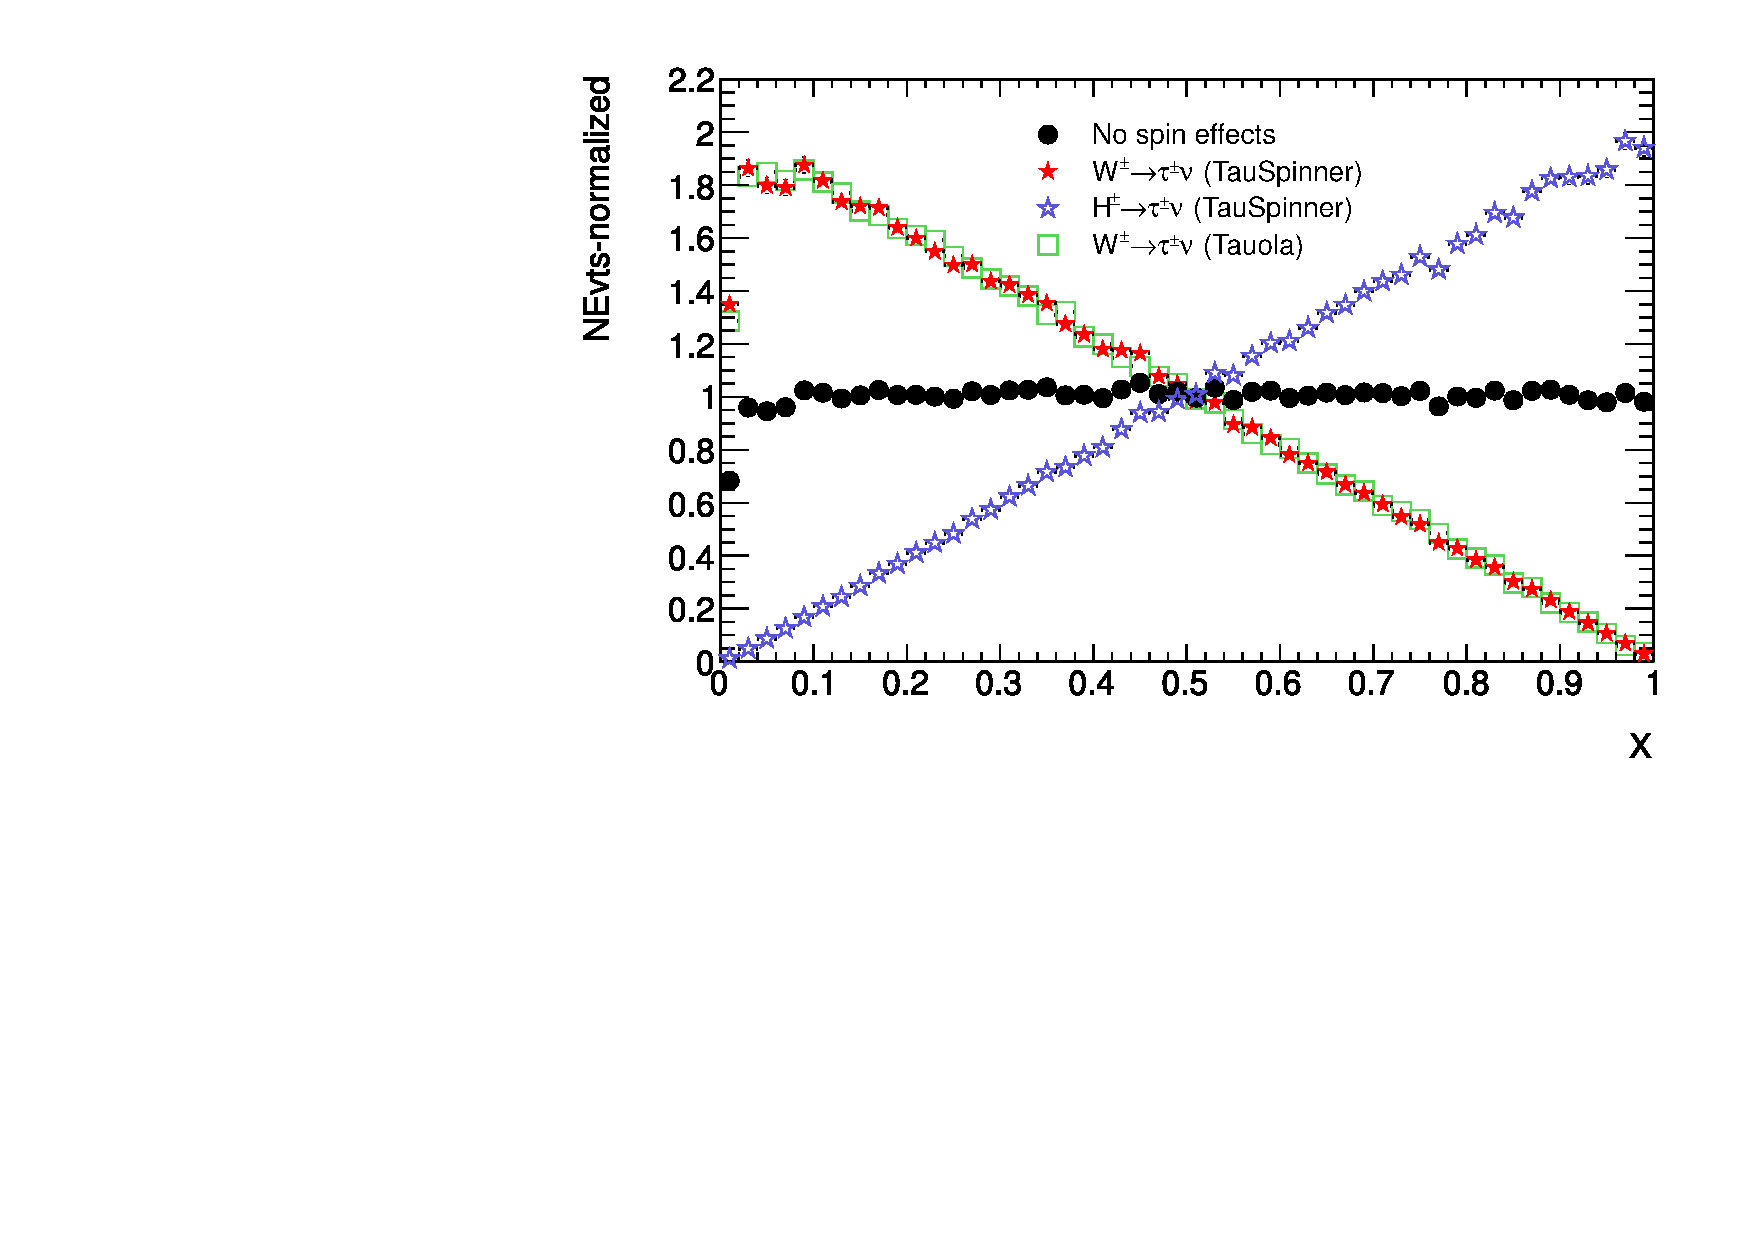
\includegraphics[width=0.5\textwidth]{figures-Tau_X_PI_}
  \label{fig:TauPolar1}
 }
 \subfigure[Relative difference between the
  charged and the neutral energy in the \RHO channel.]{
  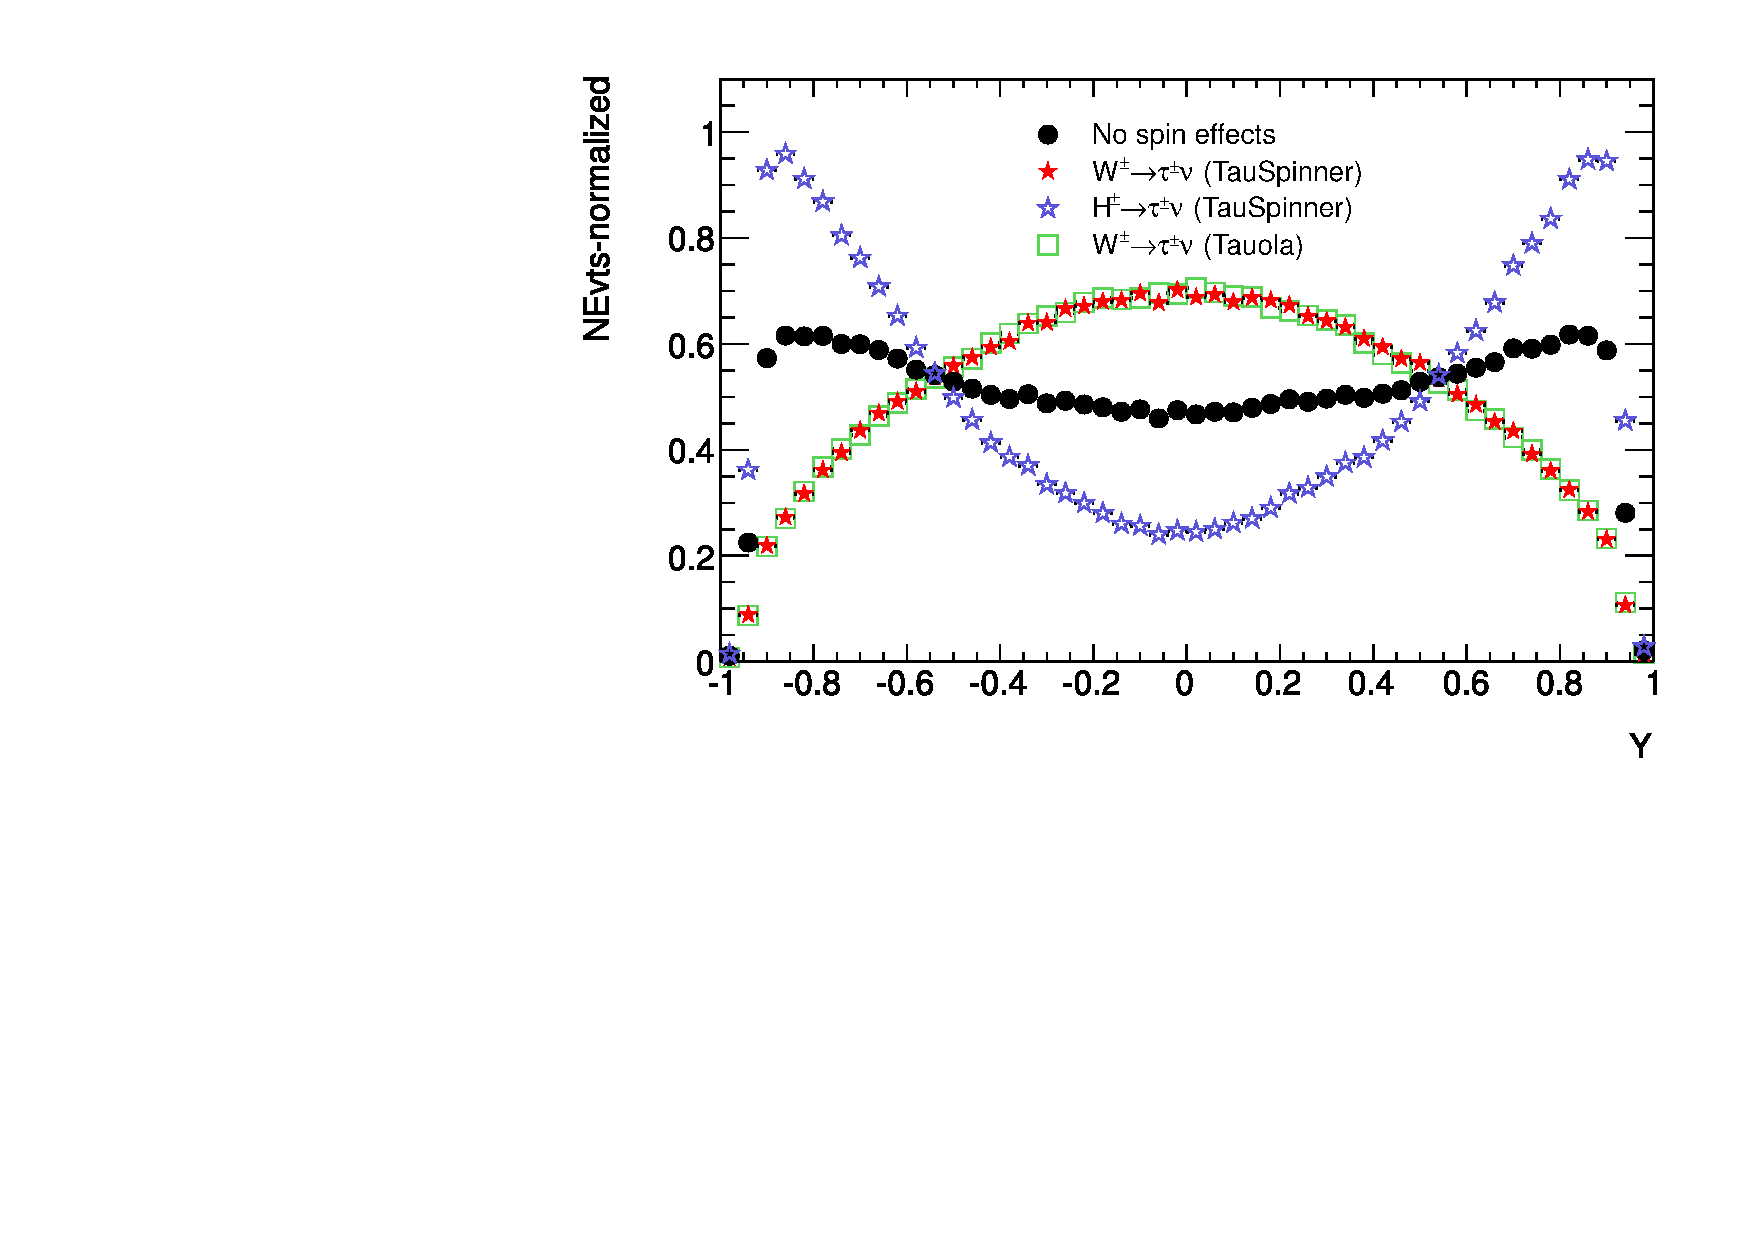
\includegraphics[width= 0.5\textwidth]{figures-Tau_Y_RHO_}
  \label{fig:TauPolar2}
 }
 \subfigure[Relative difference between the
  charged and the neutral energy in the combined \ARES and \ARESMULTI channels.]{
  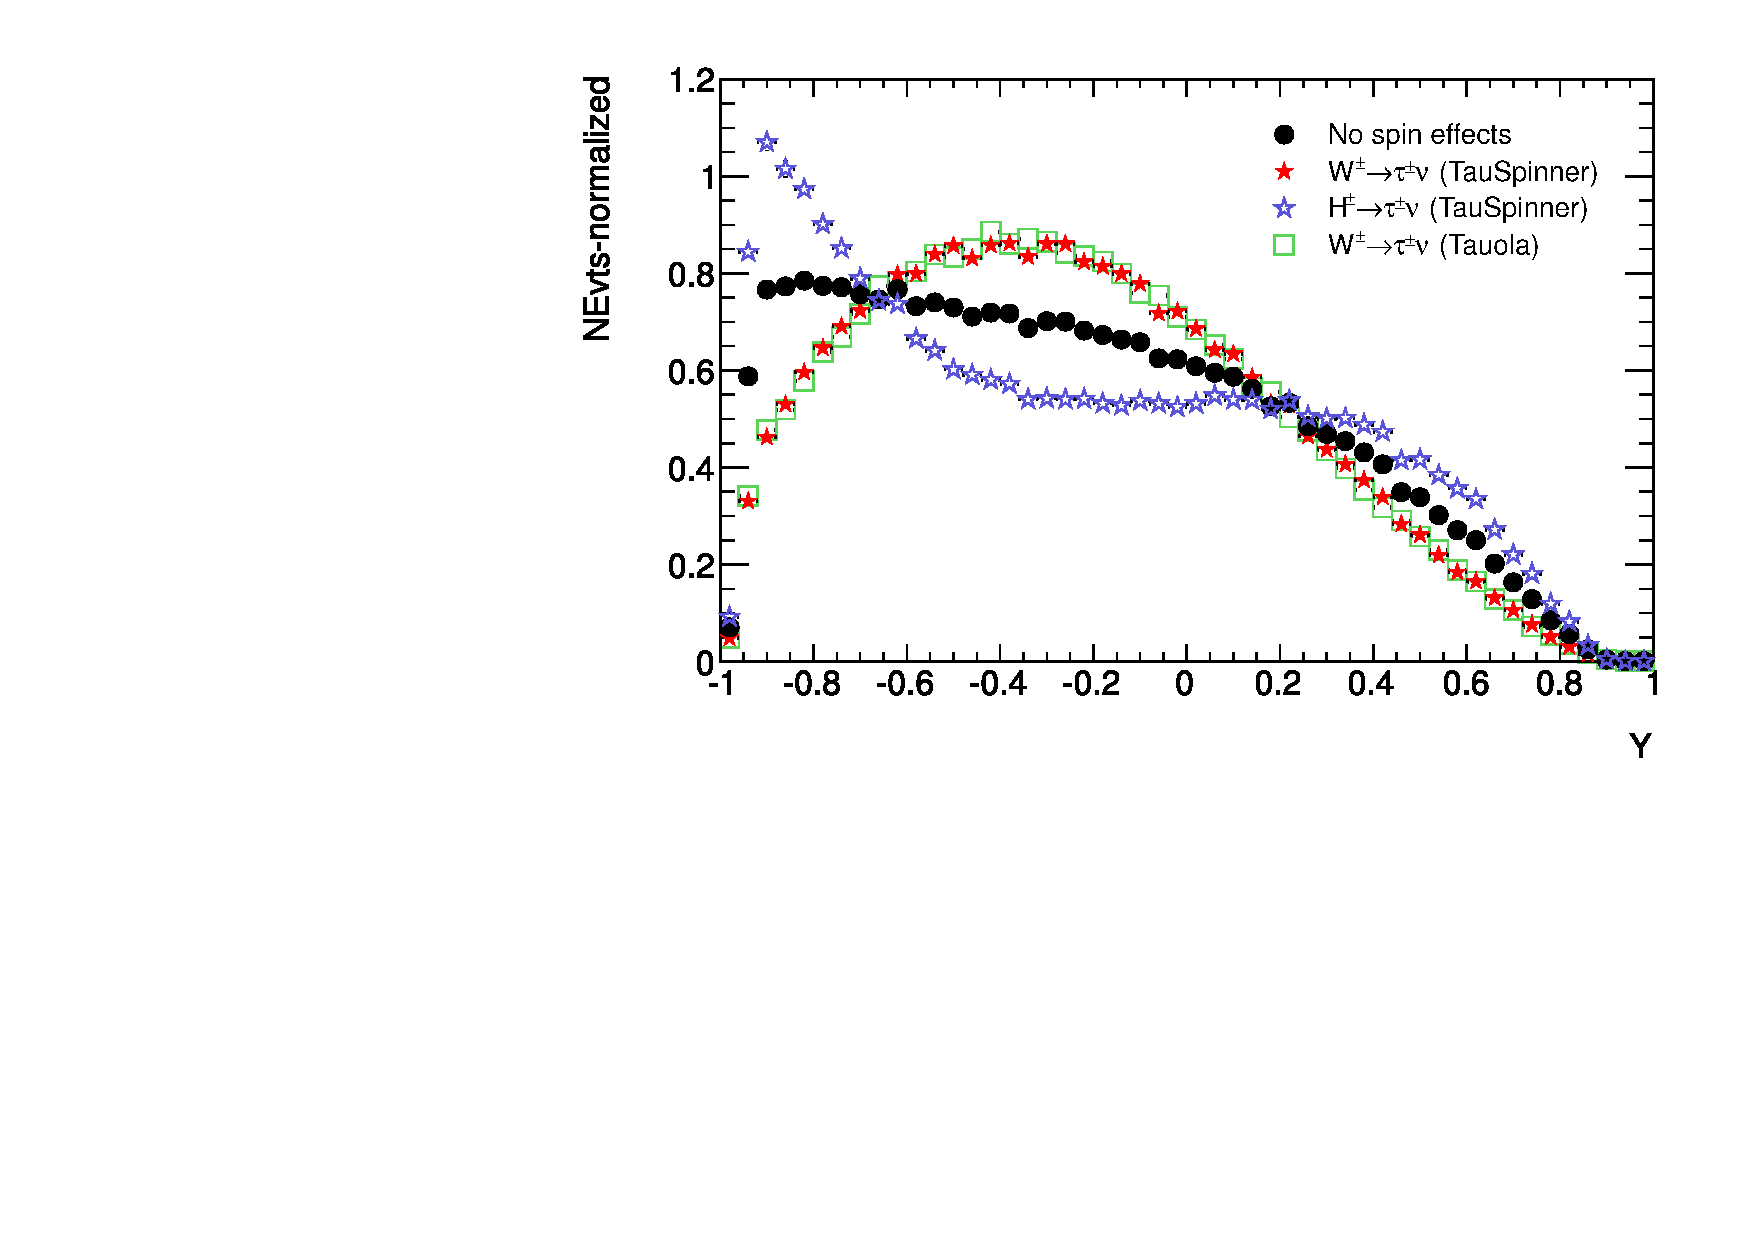
\includegraphics[width= 0.5\textwidth]{figures-Tau_Y_A1_}
  \label{fig:TauPolar3}
 }
 \caption{ Tau polarization observables }
 \label{fig:TauPolar}
\end{figure}


Note that the {\tt TauSpinner} algorithm requires that the decays of unpolarized \Tau's 
via $\rho$ or $a_1$ preserve the spin correlation between the production and decay of 
these mesons. This feature is missing if the \Tau leptons are made to decay using
{\tt Pythia}. Although a bulk of spin effects is reconstructed, a significant 
systematic uncertainty arises as demonstrated in Figure ~\ref{fig:TauPolarPythia}.


\begin{figure}
 \centering
  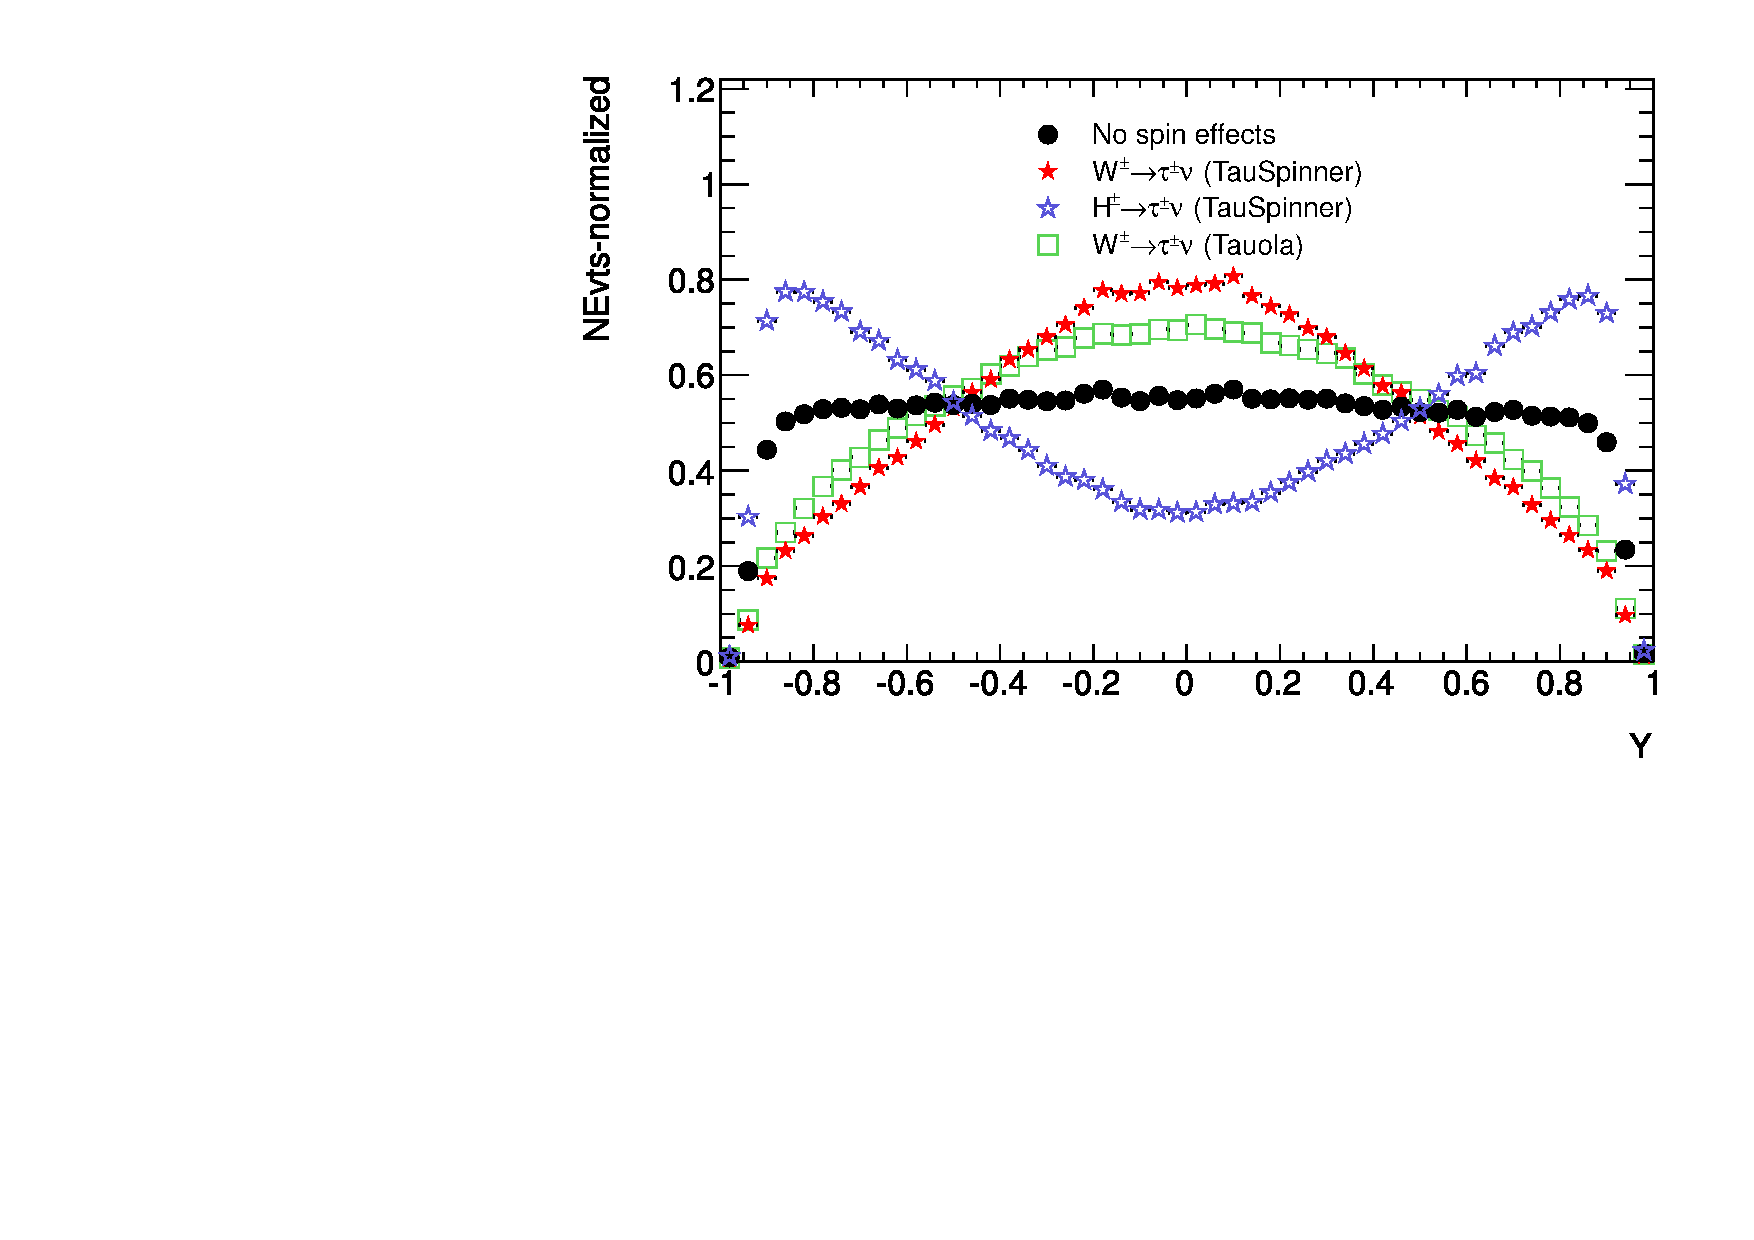
\includegraphics[width=0.5\textwidth]{figures-Tau_Y_RHO_Dziubek}
  \caption{Relative difference between the
  charged and the neutral energy in the \RHO channel. Decays of \Tau leptons in the ``no spin effects'' sample were generated using {\tt Pythia}.  
\label{fig:TauPolarPythia}}
\end{figure}



\subsection{Simulation of \Tau polarization in \Ztautau events}


In \Ztautau events, \PTAU depends on the intermediate boson virtuality,
the flavor of the incoming quark and the forward-backward asymmetry.
The complexity of this dependence is shown in
Figure~\ref{fig:TauPolCos} where the \PTAU polarization is drawn as a function 
of $cos\theta$, for two different ranges of the invariant mass of the boson.
In these plots, the quark flavor configuration is fixed at the level of simulation of the spin weight in the {\tt TauSpinner}.


\begin{figure}
 \centering
 \subfigure[\newline  The up quark aligned along the positive z axis.]{
  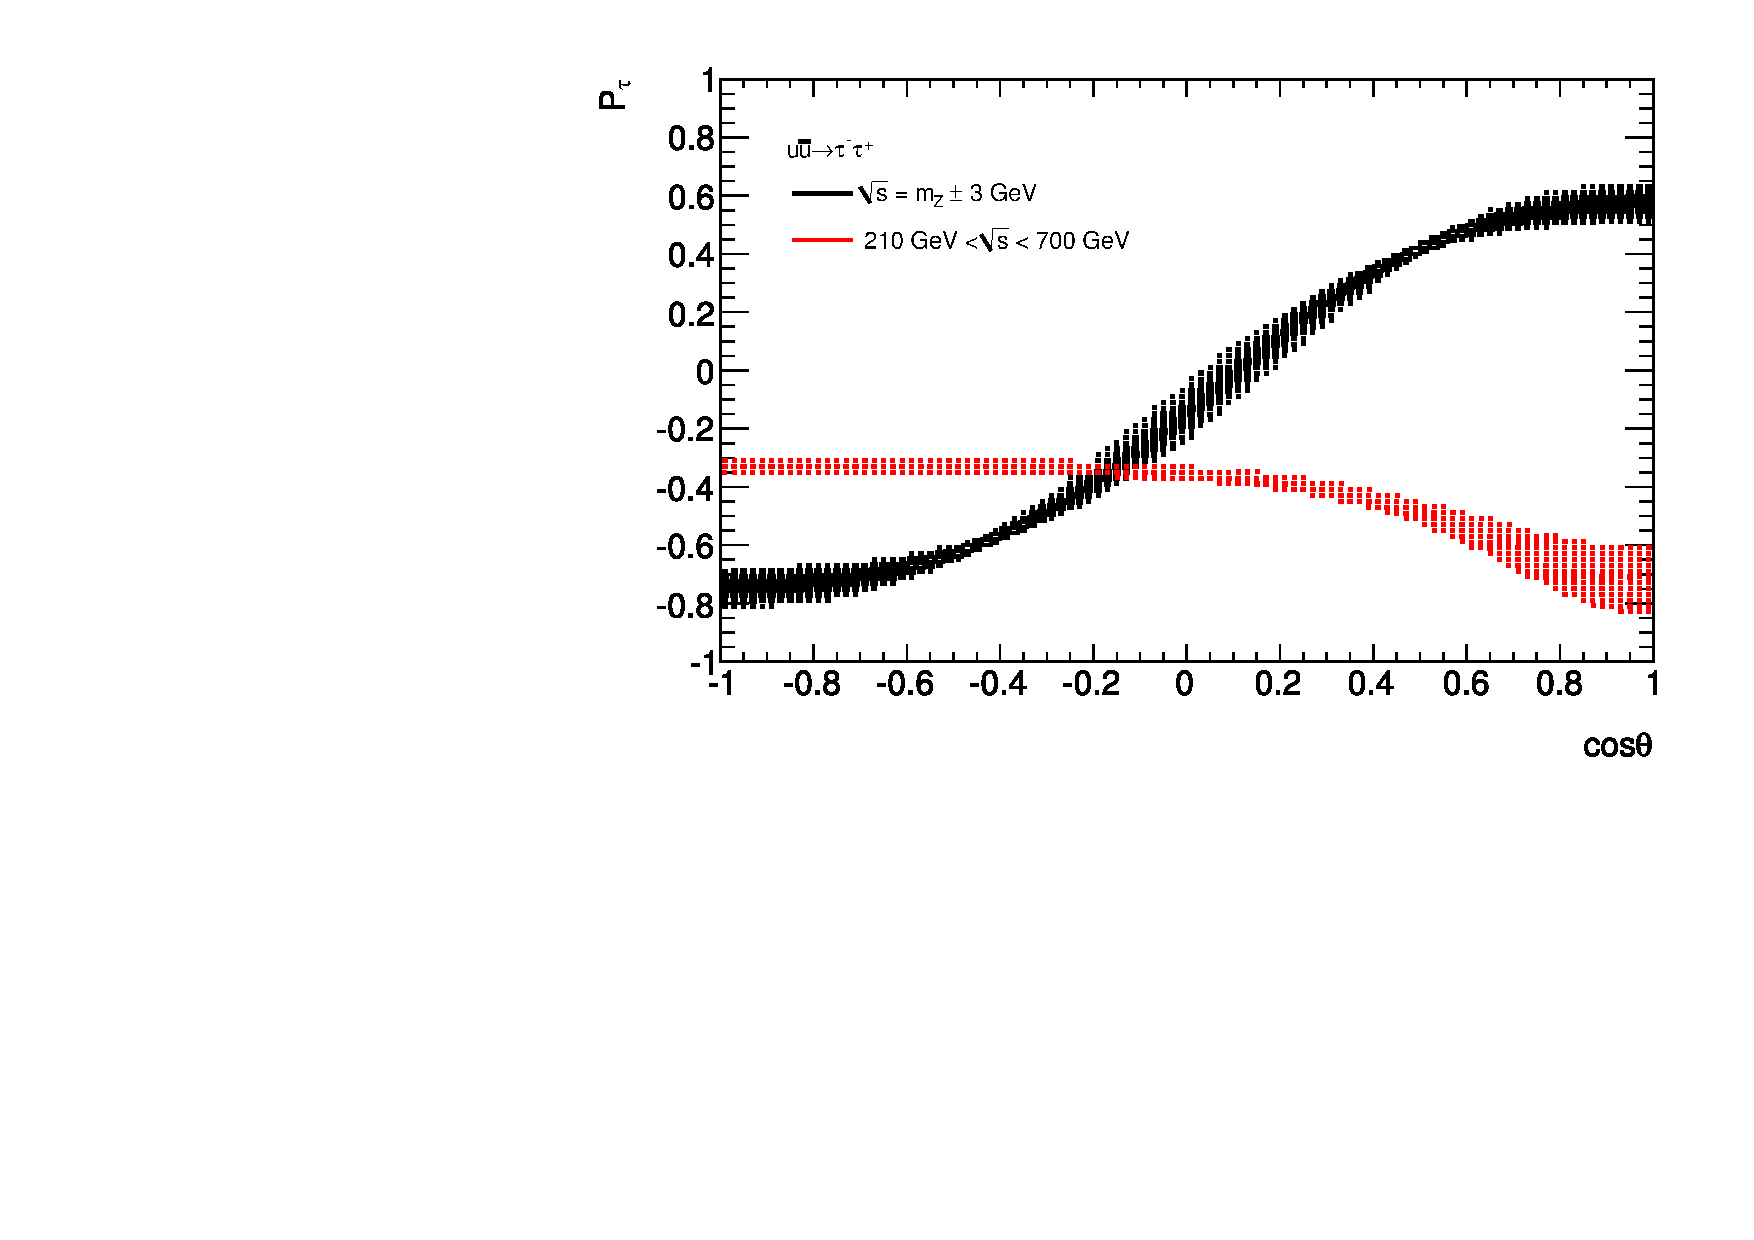
\includegraphics[scale=0.34]{figures-Ptau_cosTheta_ICC3}
  \label{fig:TauPolCos1}
 }
\hskip 1 cm
 \subfigure[\newline  The down quark aligned along the positive z axis.]{
  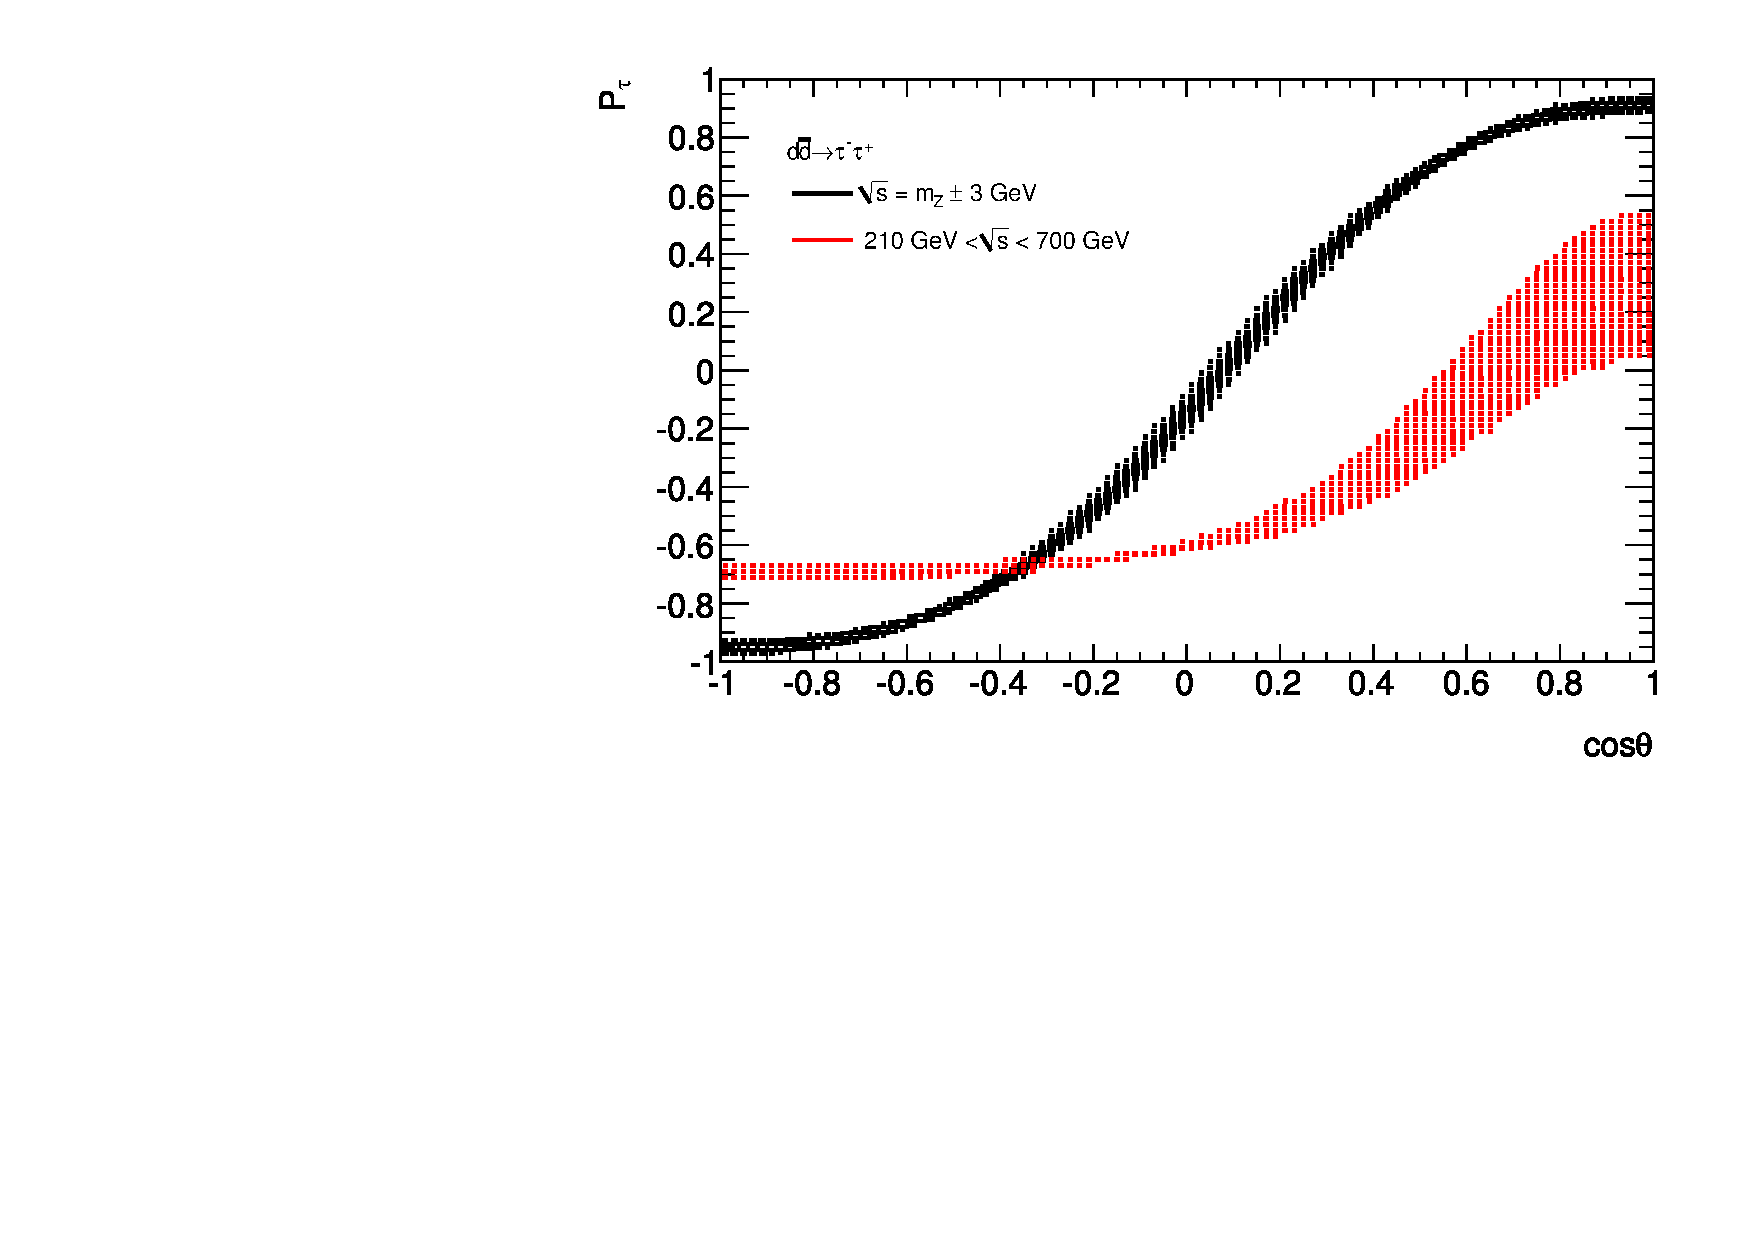
\includegraphics[scale=0.34]{figures-Ptau_cosTheta_ICC1}
  \label{fig:TauPolCos2}
 }
 \caption{\Tau polarization as a function of $cos\theta$.}
 \label{fig:TauPolCos}
\end{figure}


In the next step, a degree of polarization is studied for different configurations
of the incoming quarks. The virtuality of the intermediate boson is constrained to $M_\mathrm{Z}\pm$3 GeV
and both \Tau's are set to decay to \PI.
The forward-backward spin asymmetry is accessed by choosing the
\TauMin to be emitted in the forward region by requiring
the longitudinal momentum of \TauMin to be greater than that of \TauPlus. 
Figure~\ref{fig:XfrICC} shows the observable $x$ for the up and down type quarks
entering along the positive or negative z axis.
The results are consistent with those of reference~\cite{TauSpinERWZW},
and therefore provide assurance that a proper transmission of spin effects from the hard process
to the tau decay products is performed.


\begin{figure}
\centering 
\subfigure[\newline The up and down quarks aligned along the positive z axis.]{
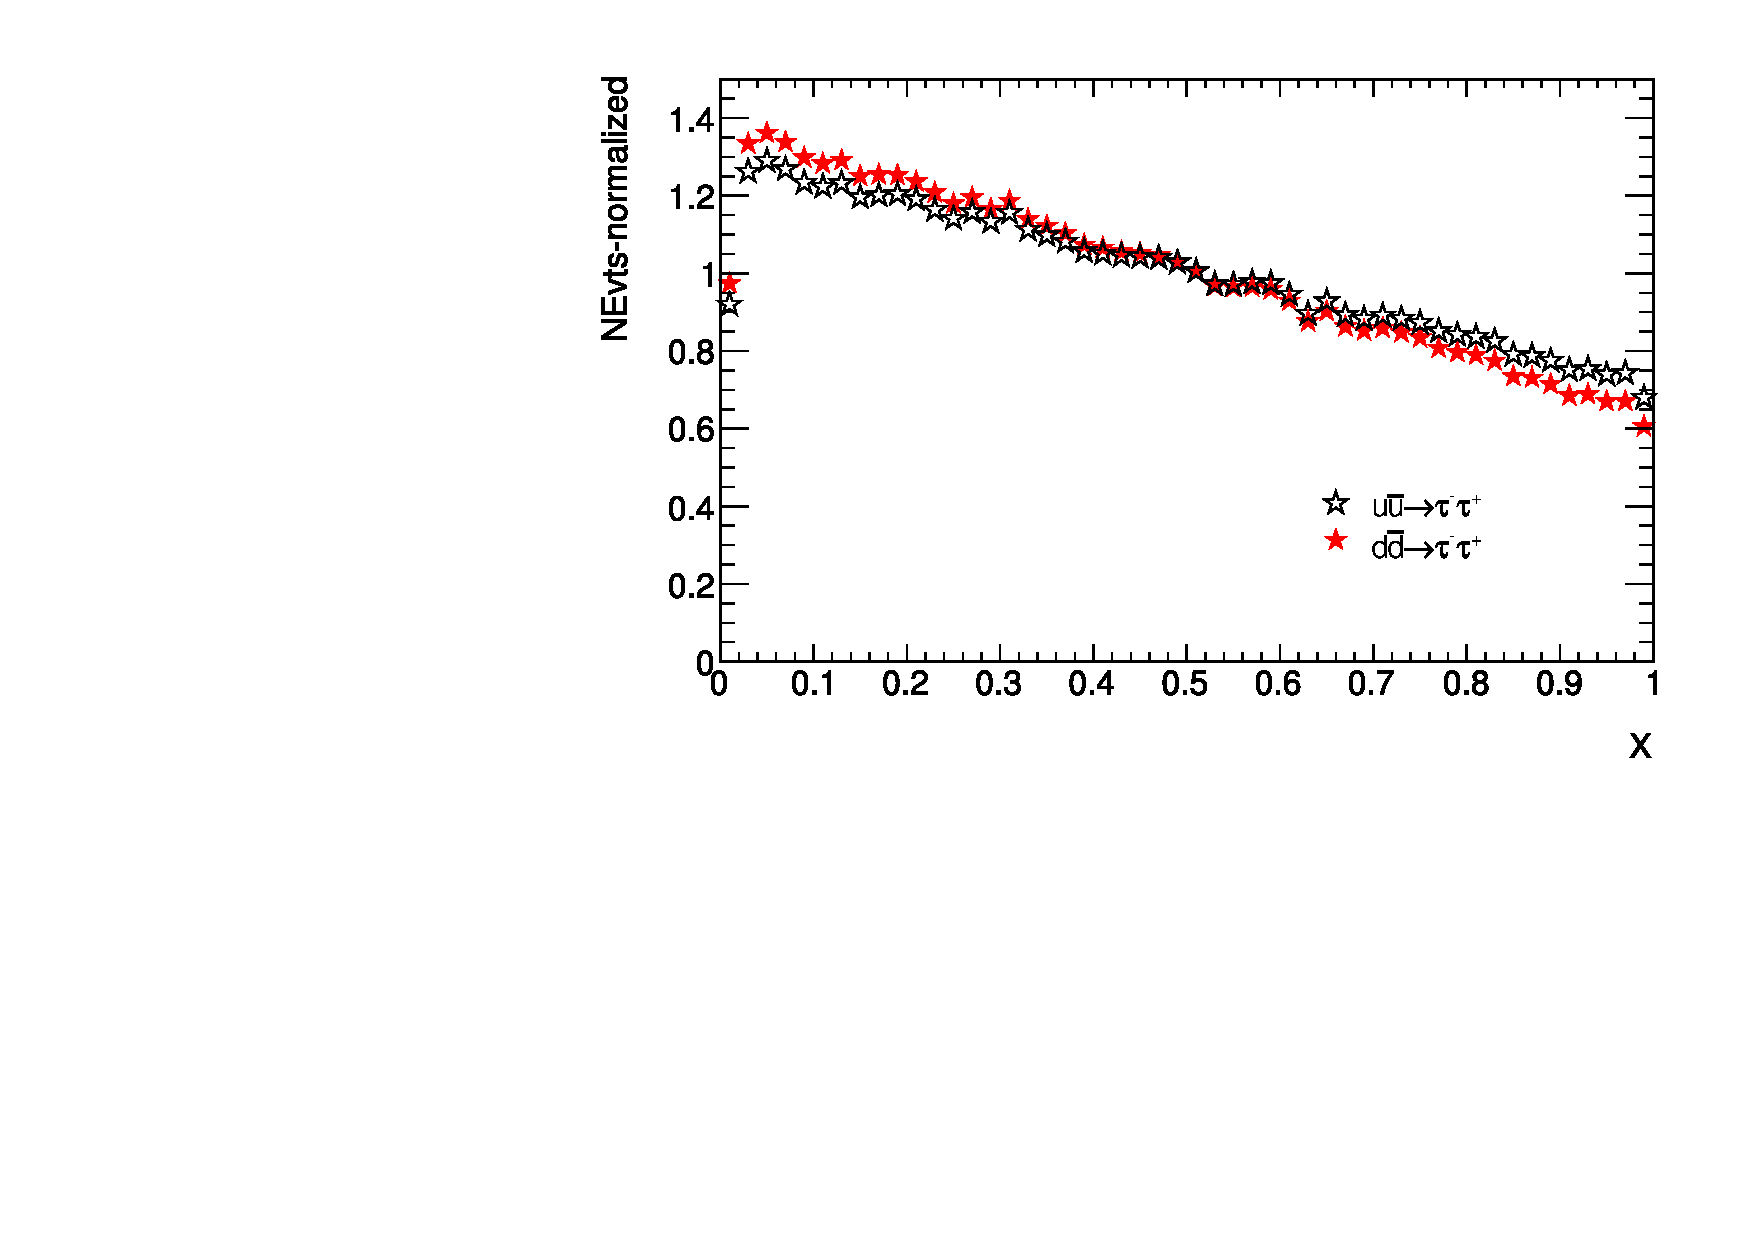
\includegraphics[scale=0.38]{figures-Xfrac_ICC0}
\label{fig:spinA}
}
\hskip 1 cm
\subfigure[\newline The up and down quarks aligned along the negative z axis.]{
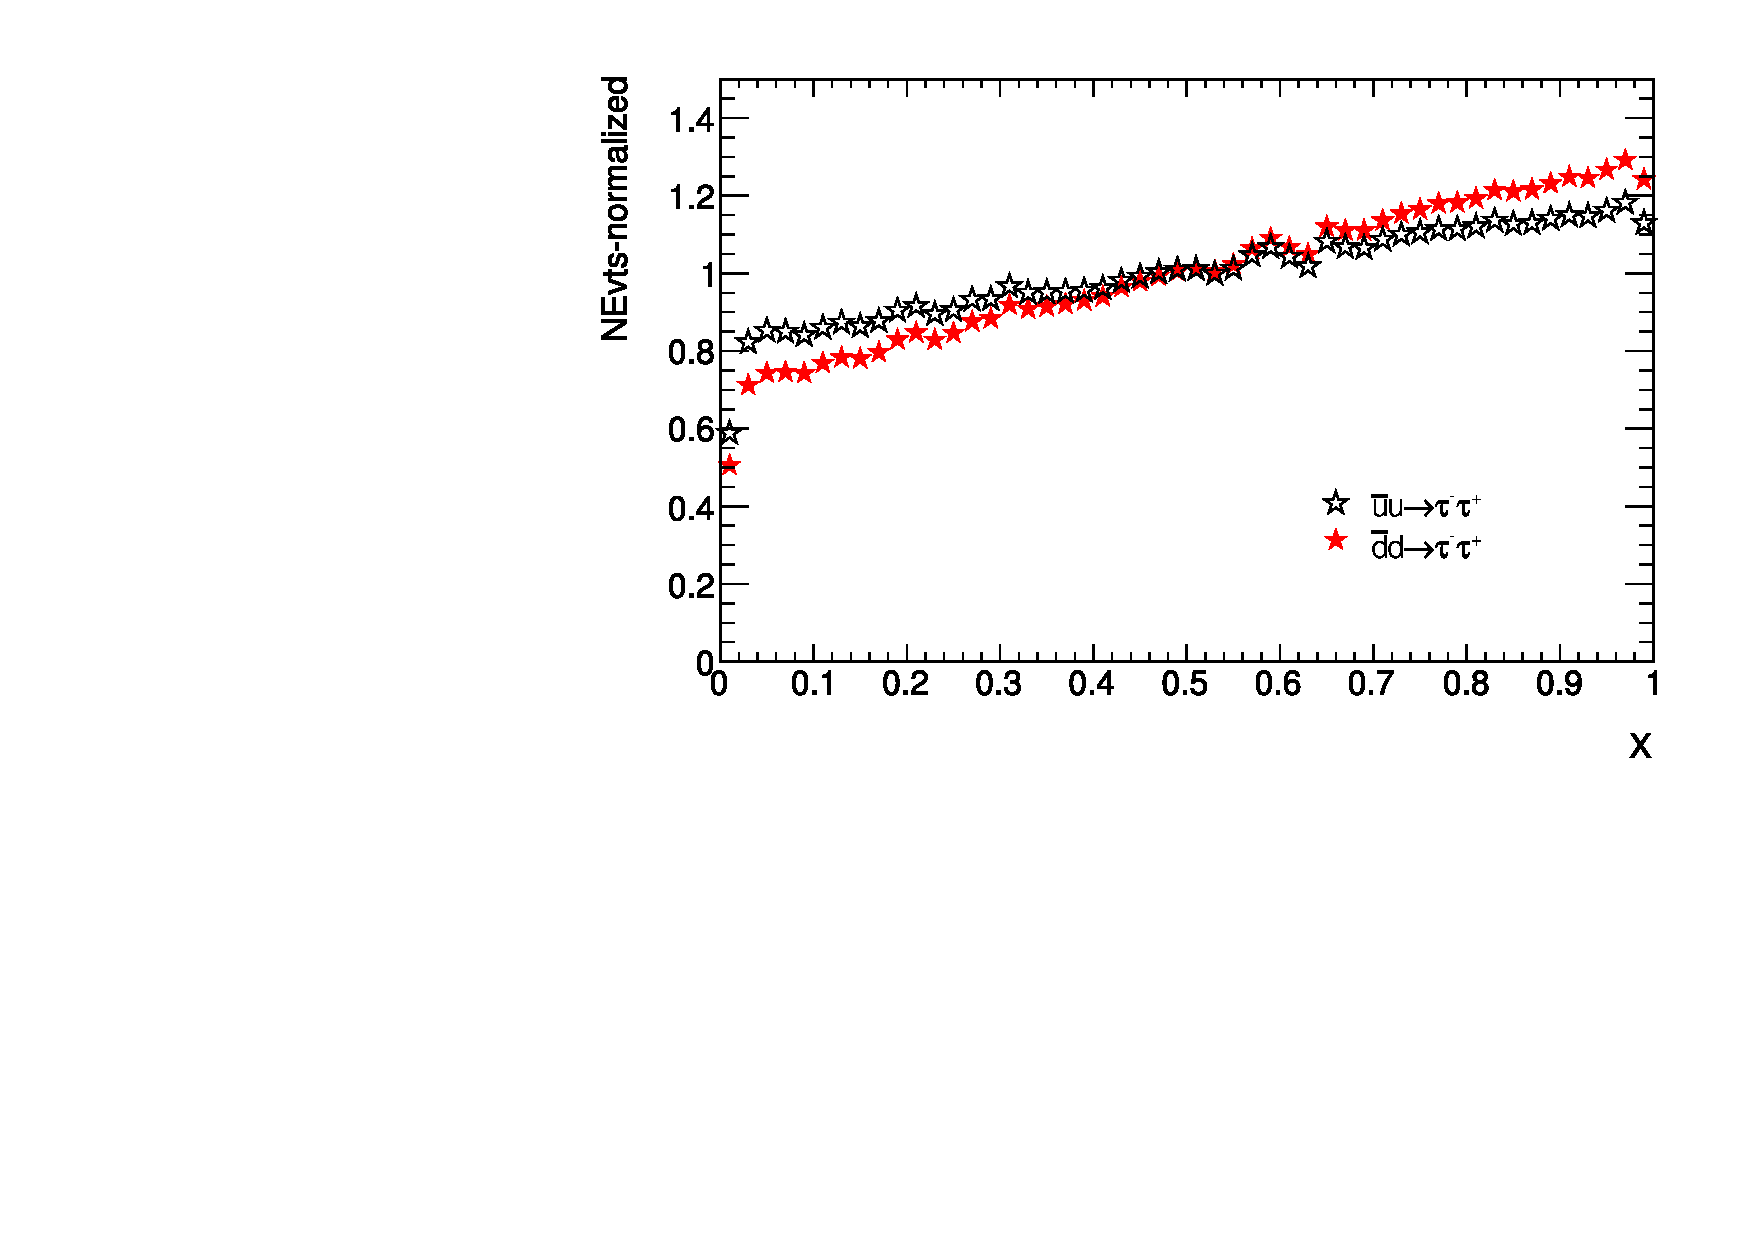
\includegraphics[scale=0.38]{figures-Xfrac_ICC1}
\label{fig:spinB}
}
\caption{
Fraction of the \Tau momentum
  taken by the hadron in the \PI channel in
  \Ztautau events.
\TauMin of forward hemisphere are chosen.
}
\label{fig:XfrICC}
\end{figure}


In the last step, the degree of polarization is
studied inclusively for all initial state quark configurations and the results are compared to
those simulated using the {\tt Tauola} package. The \ZGAMMA virtuality is constrained to $M_\mathrm{Z}\pm$3 GeV.
Fraction of the \Tau momentum taken by the hadron in the \PI
channel is plotted in Figure~\ref{fig:XfrFB}. Assuming the Z boson to 
be emitted in the direction of the incoming quark ( as compared to the
direction of the anti-quark ) these plots can be compared to those in Figure~\ref{fig:XfrICC}.


\begin{figure}
 \centering
\subfigure[  Z boson emitted \newline  \; in the forward direction.]{
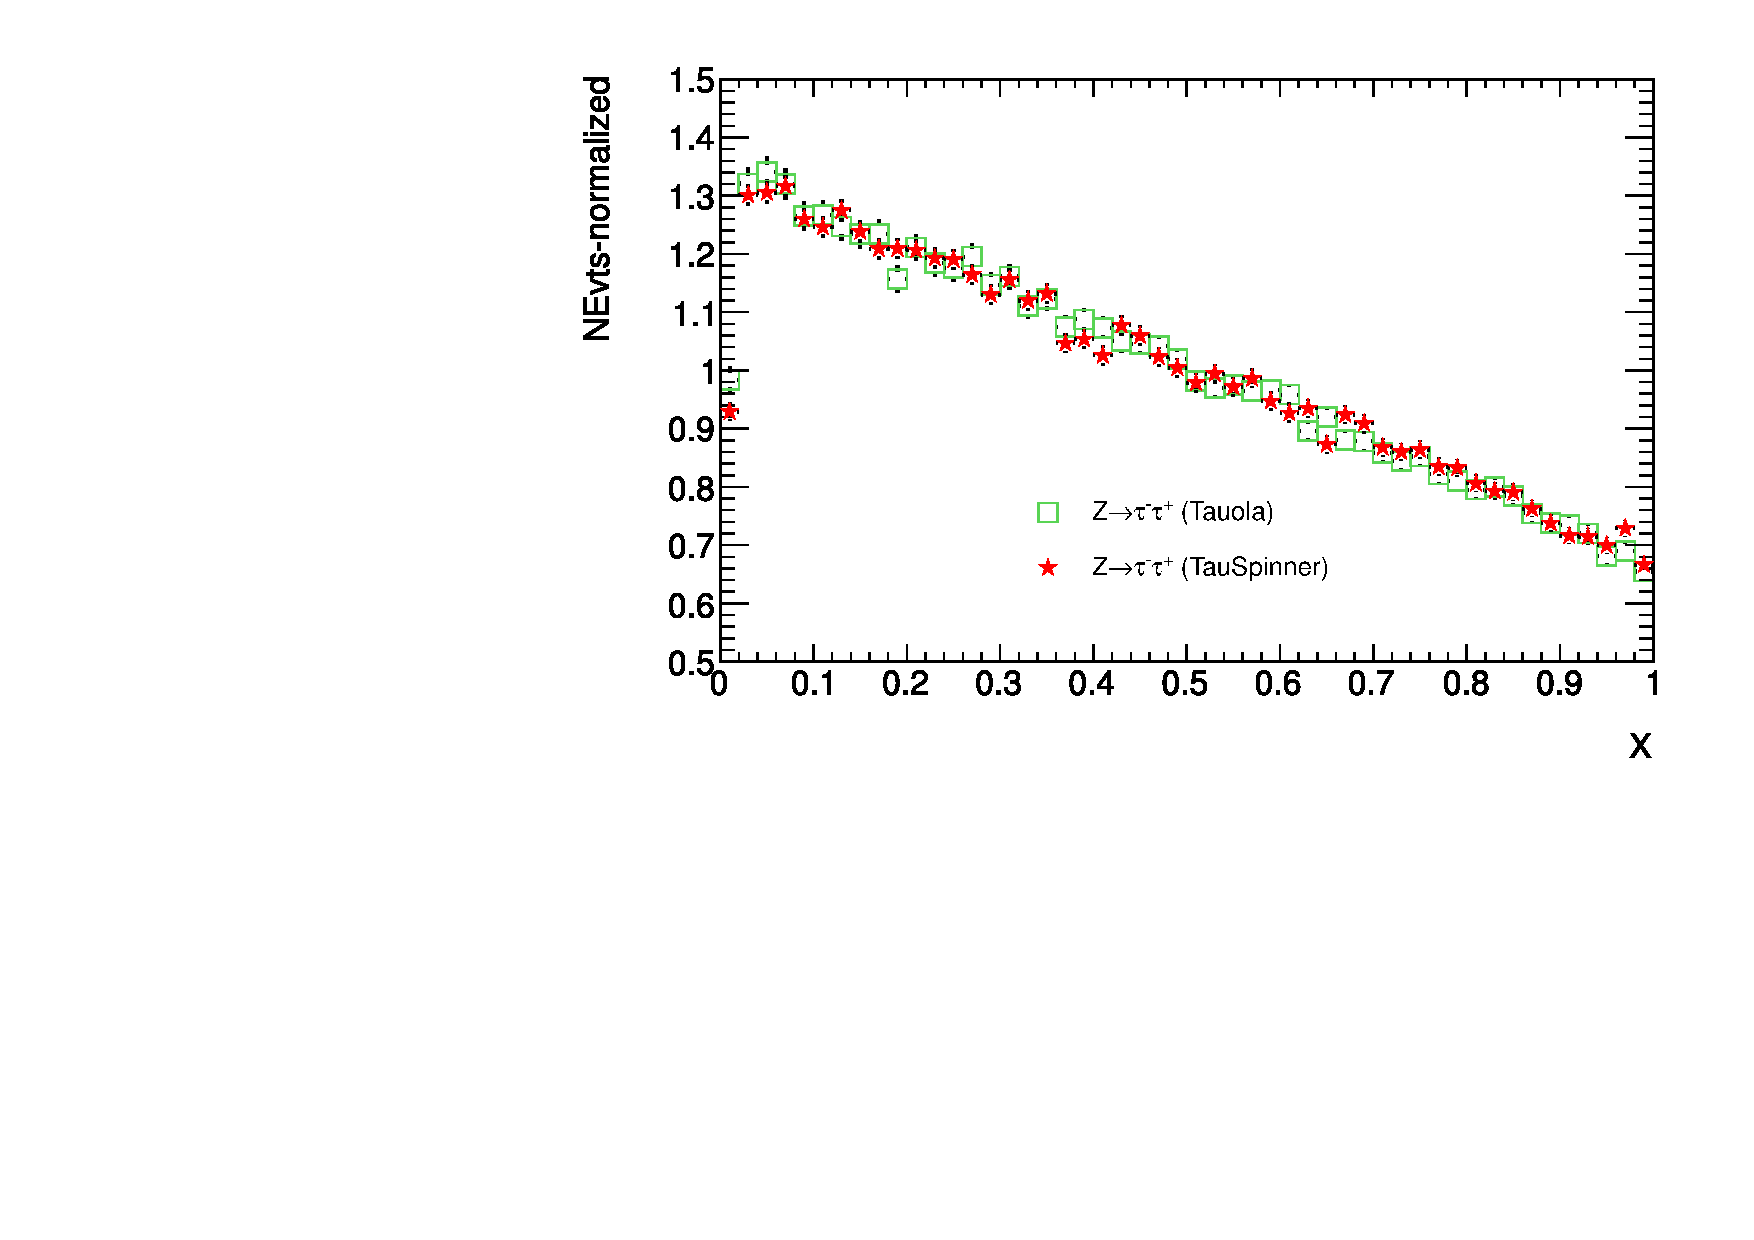
\includegraphics[scale=0.38]{figures-Tau_X_F_}
\label{fig:spinA1}
}  \hskip 1 cm 
%\hskip 1 cm  \vskip 
\subfigure[  Z boson emitted  \newline in the backward direction.]{
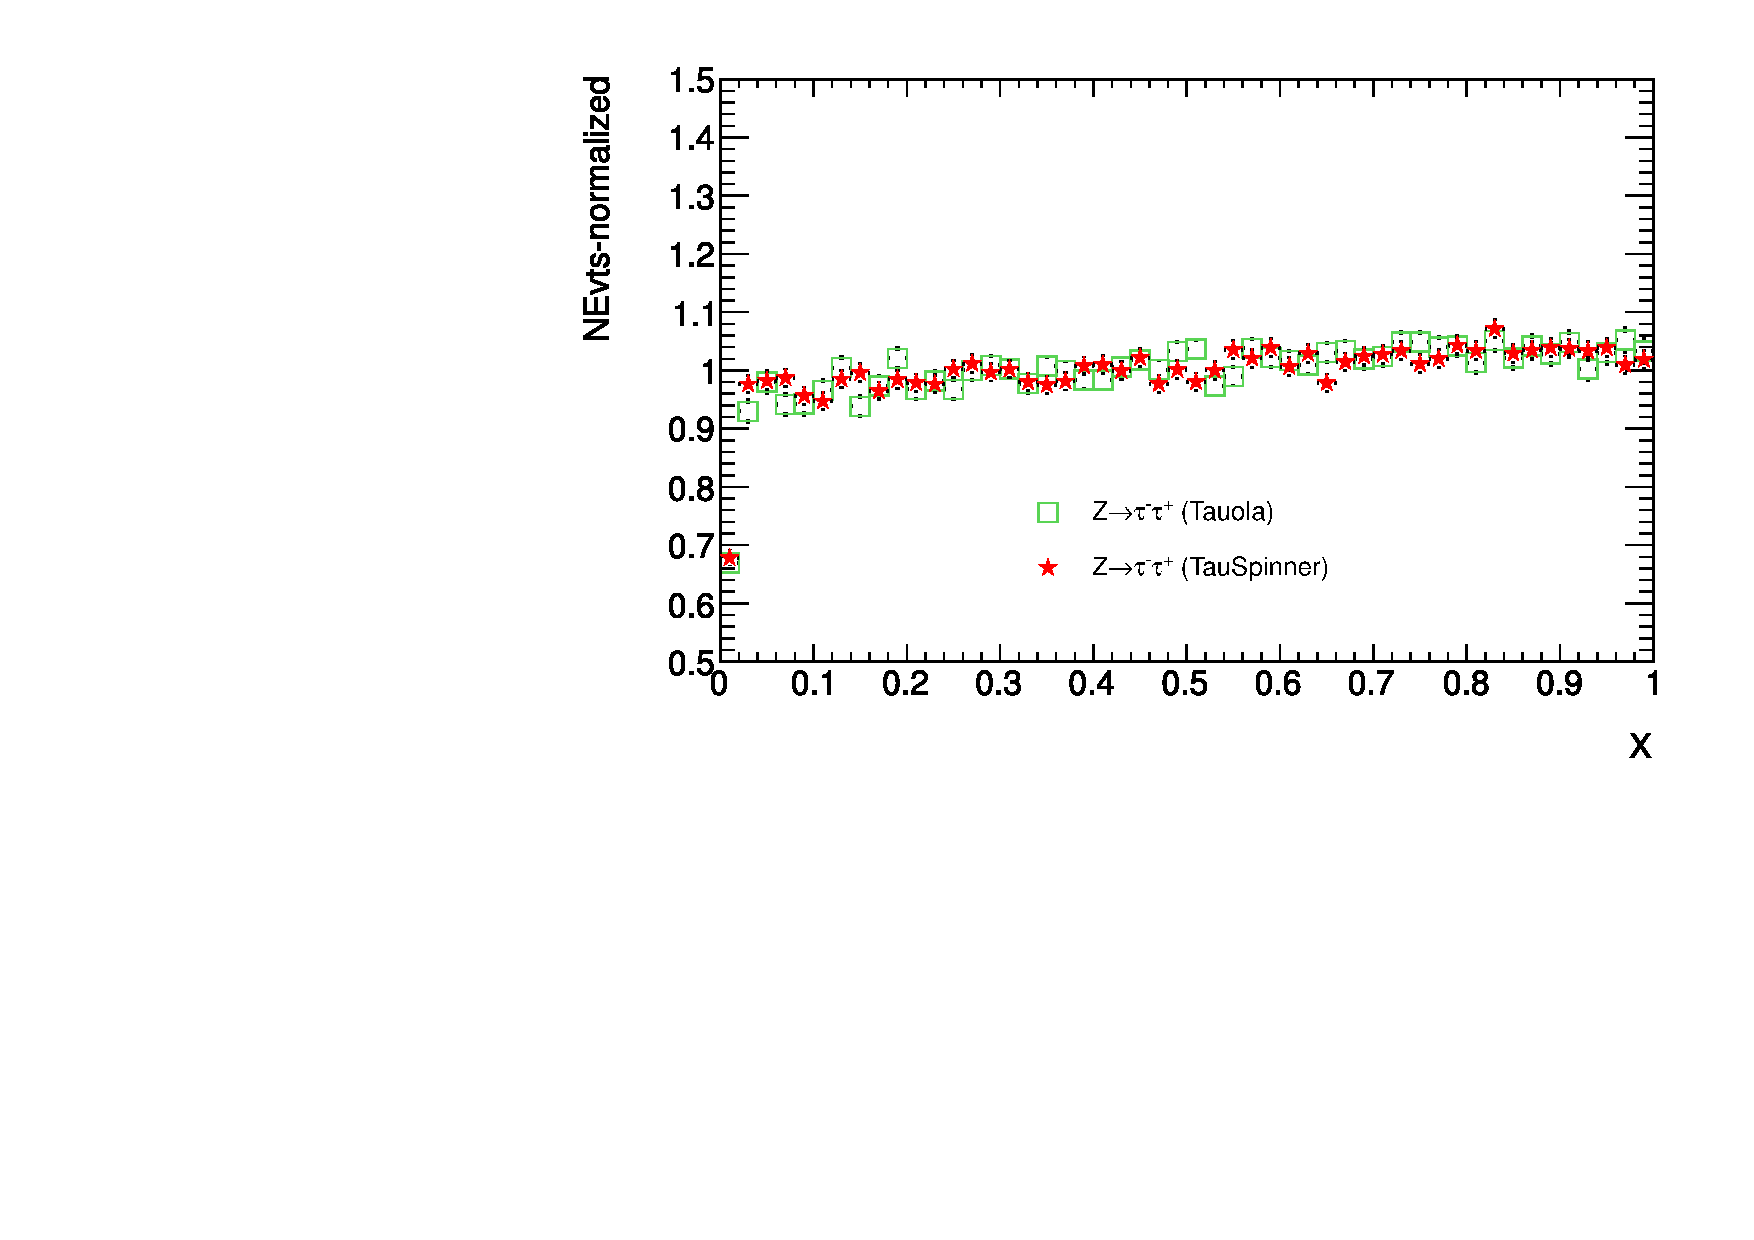
\includegraphics[scale=0.38]{figures-Tau_X_B_}
\label{fig:spinB1}
}
\caption{
Fraction of the \Tau momentum taken by the hadron in the \PI 
channel. \TauMin of forward hemisphere are chosen.
}
\label{fig:XfrFB}
\end{figure}



\subsection{Validation of spin correlation in the \TauTau final
state}


Two observables were demonstrated in~\cite{TauSpinERWZW} to be appropriate for studying 
of \Tau lepton spin correlations in the \Tau-pair final state: the
invariant mass of the hadronic system and the z$_s$ variable.
The latter is a signed surface in $x^+$, $x^-$ plane, between 
lines: $x^+$=$x^-$ and $x^+$=$x^-$+a. The $x^+$ and $x^-$ 
denote the fraction of \Tau momenta taken by the hadrons.
The two observables are plotted in Figure~\ref{fig:TauCorr}
in the channel where both \Tau leptons decay to \PI.
The sample with no spin effects refers to \Ztautau events generated
with a flat \PTAU value. The proper \Htautau and \Ztautau configurations were obtained by applying an
appropriate spin weight to the sample with no spin effects.
The weighed observables exhibit the expected behavior
reassuring a proper implementation of the spin correlations in the {\tt TauSpinner} package.


\begin{figure}
% \centering
 \subfigure[ The z$_s$ variable described in text in the channel where both
 \Tau leptons decay to \PI.]{
  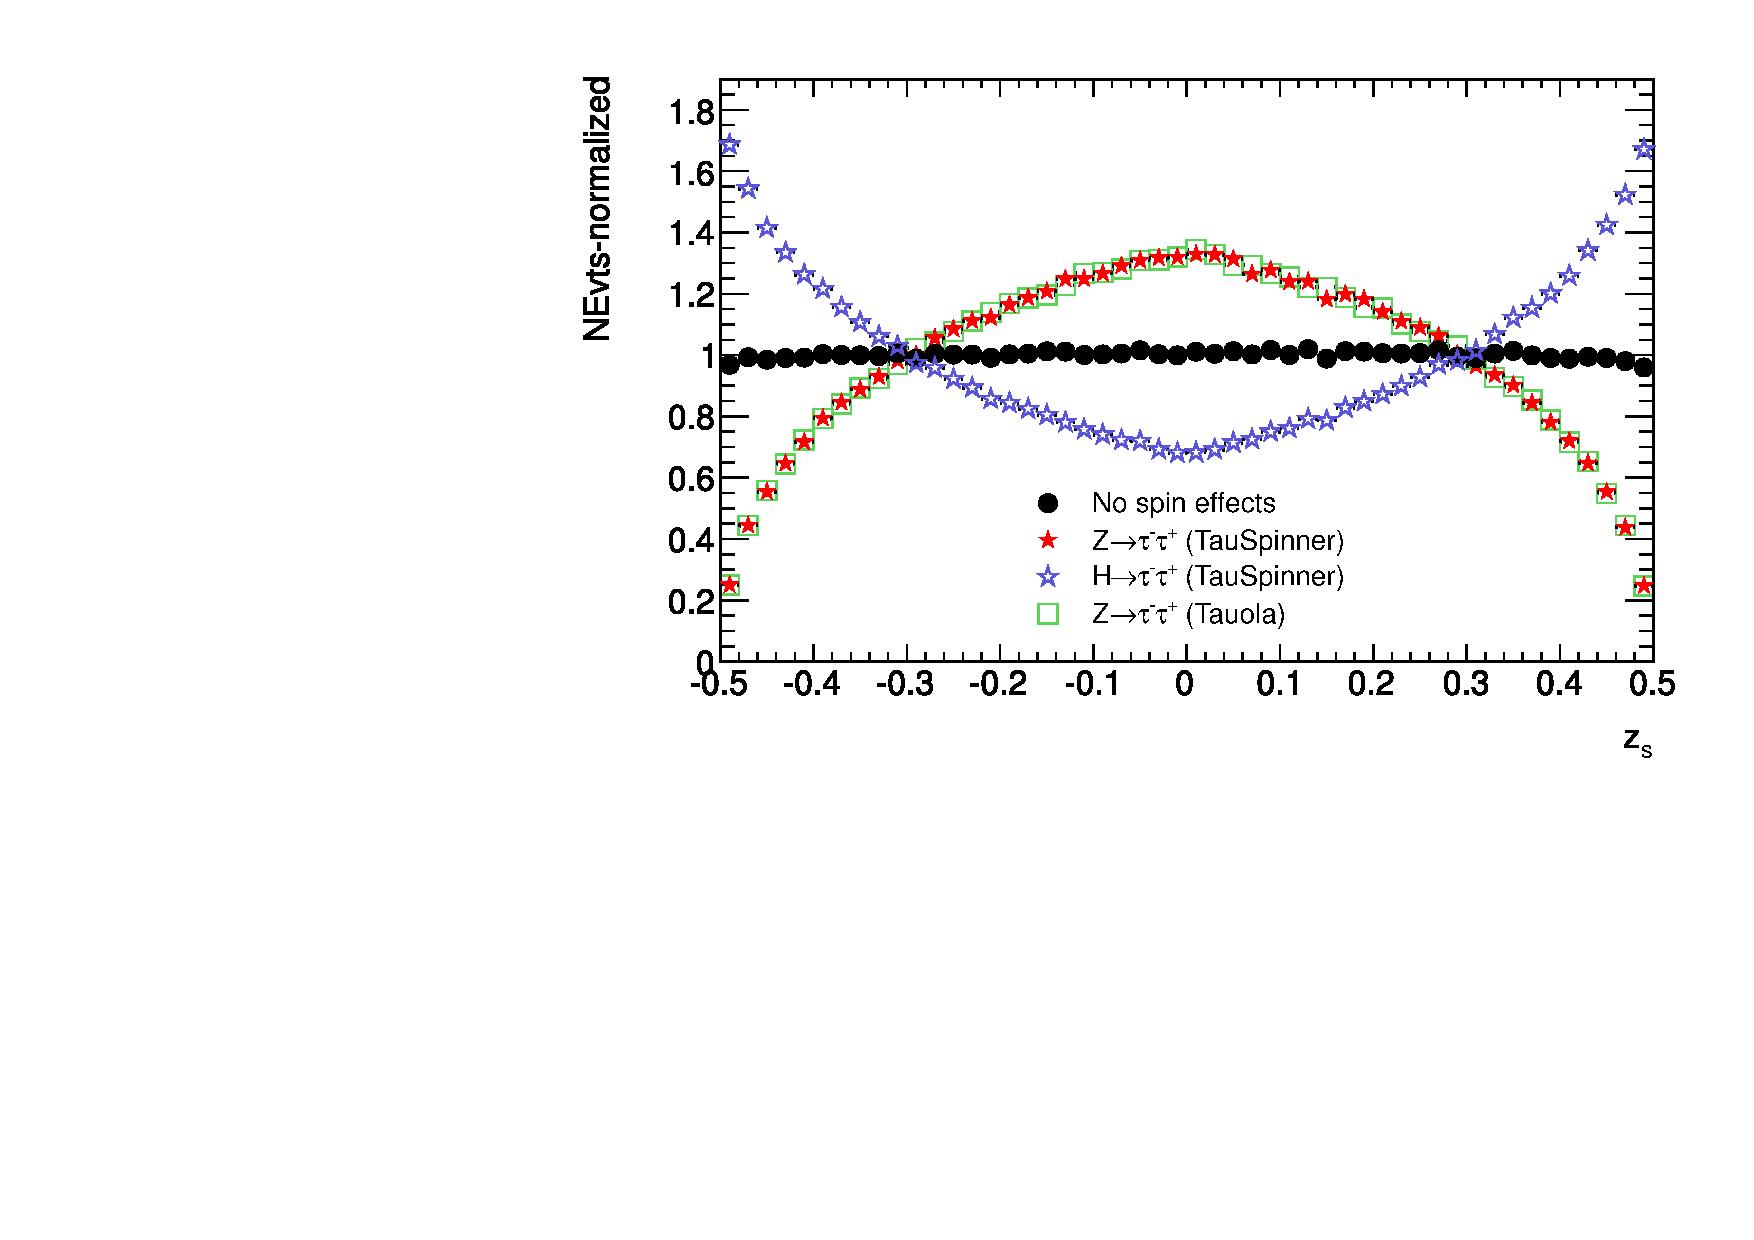
\includegraphics[scale=0.38]{DiTau_ZS_X_}
  \label{fig:TauCorr1}
 }
\hskip 1 cm 
 \subfigure[ \; \newline Visible mass of the two hadrons in the channel where both
 \Tau leptons decay to \PI.]{
  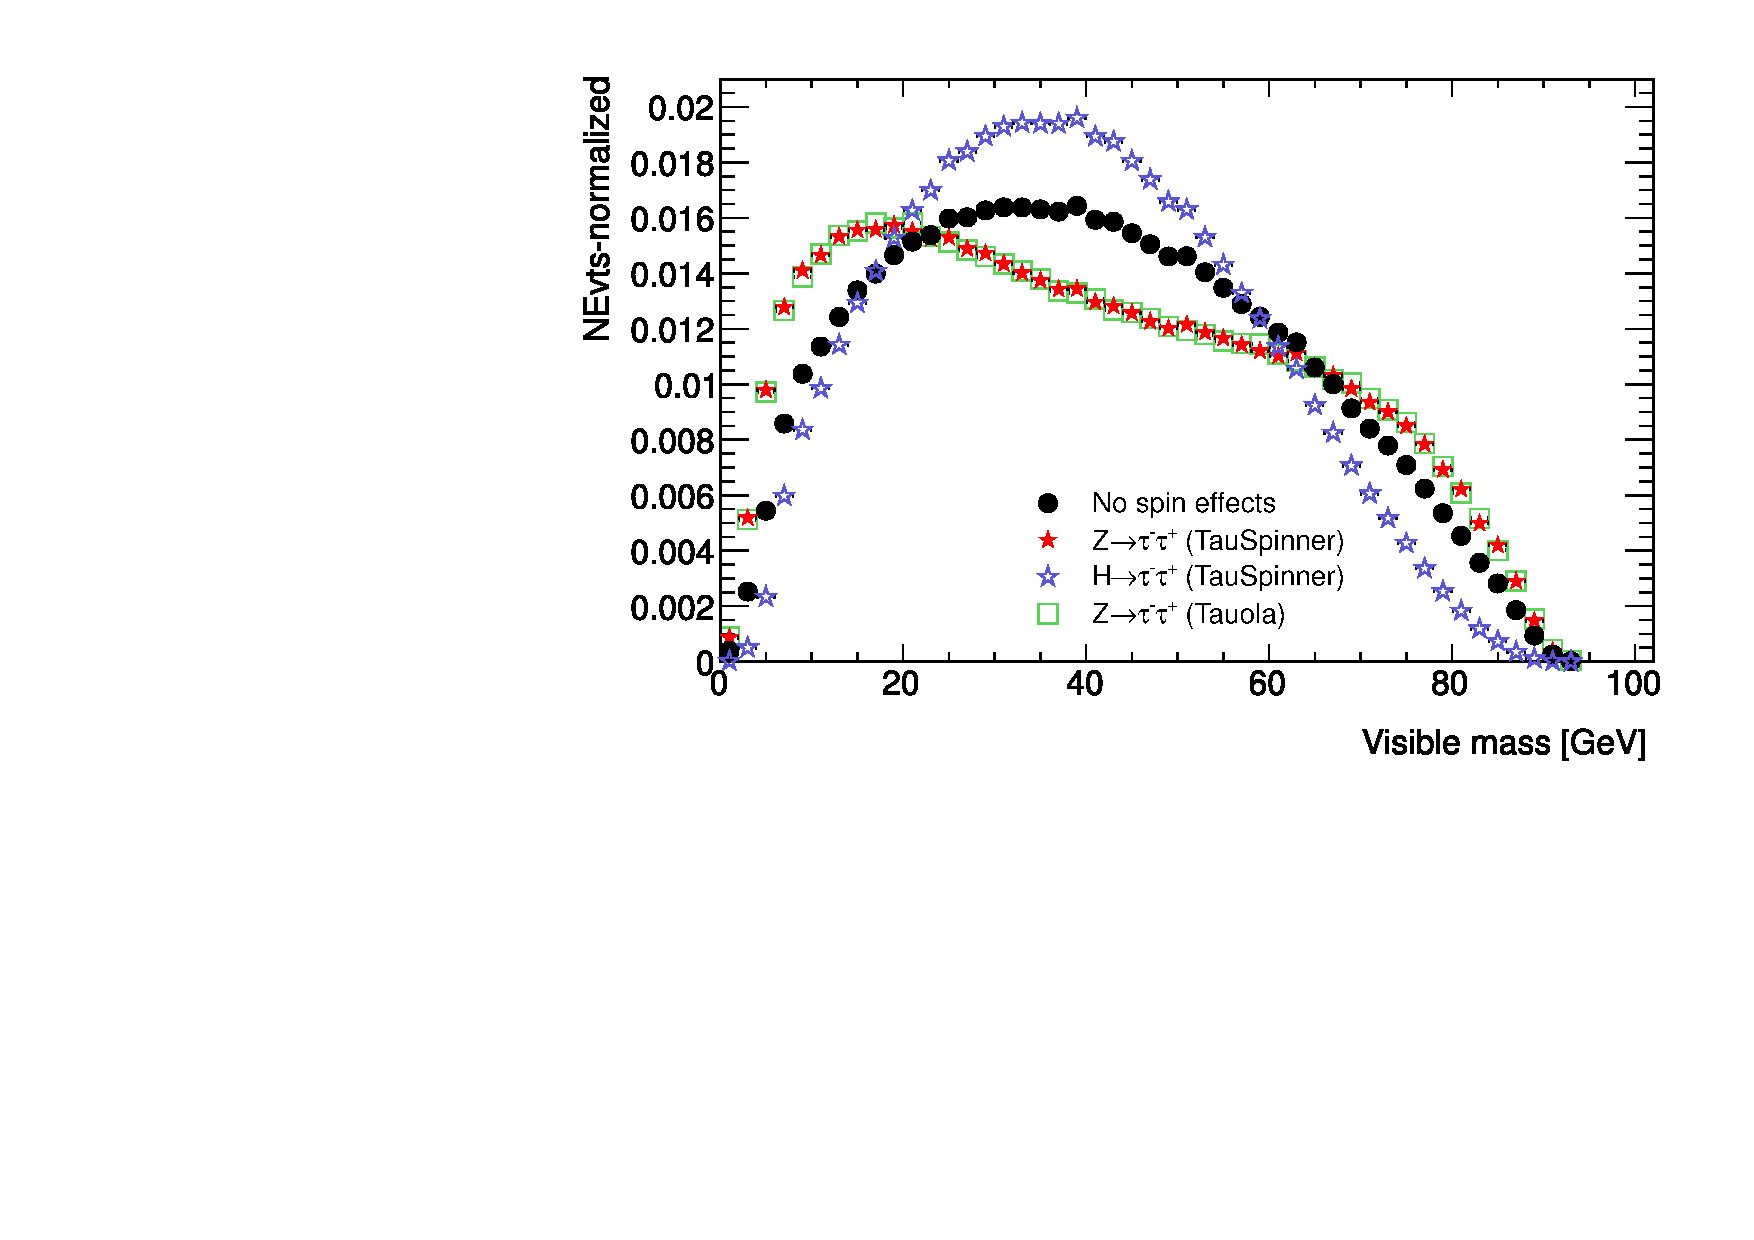
\includegraphics[scale=0.38]{DiTau_MVis_}
  \label{fig:TauCorr2}
 }
 \caption{\Tau spin correlation observables.}
 \label{fig:TauCorr}
\end{figure}


\section{Summary and outlook}\label{sect:Summary}


The {\tt TauSpinner} package designed to emulate \Tau spin effects has
been introduced. The algorithm is limited to the leading order accuracy and
the longitudinal spin degrees only. As compared to the algorithm developed in~\cite{TauSpinERWZW}, the
functionality is extended to allow one to estimate the spin effects when the
information on the incoming quarks entering the hard process is not
available. The intrinsic \Tau polarization arising from parity violation in the weak interactions
is attributed on the basis of intermediate boson kinematics and PDF's.
For the \Ztautau process its complete functionality is limited to proton-proton collisions
and otherwise restricted to conservation of total angular momentum. 
This is the first algorithm suitable for emulating of the spin effects
in the $\tau$-embedded samples.


Comparisons of {\tt Tauola} and {\tt TauSpinner} for various spin observables
presented in Section~\ref{sect:Perf} demonstrate 
that no additional systematic uncertainty in simulation of 
\Tau spin effects have been introduced in the {\tt TauSpinner}. 
This conjecture should, however, be validated in a sample
where the number of high $p_T$ jets is enhanced.


A complete discussion of the theoretical uncertainties
is common for the {\tt Tauola}, the {\tt TauSpinner} and to a large extent
the KORALZ~\cite{Jadach:1993yv} Monte Carlo programs.
Some aspects of these uncertainties have been address through
the work published in~\cite{TAUOLA1,TAUOLA2,TAUOLA3,Jadach:1984iy,Jadach:1999vf,vanHameren:2008dy}.
A rigorous evaluation of theoretical effects and in particular a comparison
with results based on the next-to-leading order matrix element calculations
simultaneous for scattering processes and
for spin density matrices is referred to a future work.


The code of {\tt TauSpinner} is publicly available
\footnote{http://wasm.web.cern.ch/wasm/newprojects.html},
with all relevant details given in
Appendix B. 

\vskip 2 mm
\centerline{\bf Acknowledgments}
\vskip 2 mm
We would like to thank A. Buckley, S.Demers, C. Gwenlan, E. Richter-Was and S. Tsuno
for valuable discussions. \\
{ The work of Tomasz Przedzinski was supported in
 part by the Polish Government grant NN202127937 (years 2009-2011).}

\providecommand{\href}[2]{#2}\begingroup\raggedright\begin{thebibliography}{10}

\bibitem{EMBEDDED}
{Atlas collaboration}, {\em {Search for neutral MSSM Higgs bosons decaying to
  $\tau^{+}\tau^{-}$ pairs in proton-proton collisions at sqrt(s) = 7 TeV with
  the ATLAS detector}\/},  Phys. Lett. {\bf B 705} (2011)  174--192.

\bibitem{TAUOLA1}
S.~Jadach et al.
Comput. Phys. Commun. {\bf 64} (1990)  275.
%%CITATION = NUPHA,22,579;%%.

\bibitem{TAUOLA2}
M.~Jezabek et al.
Comput. Phys. Commun. {\bf 70} (1992)  69.
%%CITATION = NUPHA,22,579;%%.

\bibitem{TAUOLA3}
R.~Decker et al.
Comput. Phys. Commun. {\bf 76} (1993)  361.
%%CITATION = NUPHA,22,579;%%.

\bibitem{TauSpinERWZW}
T.~Pierzchala et al., {\em {Spin effects in tau lepton pair production at
  LHC}\/},
Acta Physics Polonica {\bf B32} (2001)  1277--1296.
%%CITATION = NUPHA,22,579;%%.

\bibitem{Davidson:2010rw}
N.~Davidson, G.~Nanava, T.~Przedzinski, E.~Richter-Was, and Z.~Was, {\em
  {Universal Interface of TAUOLA Technical and Physics Documentation}\/},
  \href{http://arxiv.org/abs/1002.0543}{{\tt arXiv:1002.0543 [hep-ph]}}.

\bibitem{Jadach:1984iy}
S.~Jadach and Z.~Was, {\em {Monte Carlo Simulation of the process
  $e^{+}e^{-}\rightarrow \tau^{+}\tau^{-}$ including radiative O($\alpha^{3}$)
  QED corrections, mass and spin}\/},
  \href{http://dx.doi.org/10.1016/0010-4655(85)90123-7}{Comput.Phys.Commun.
  {\bf 36} (1985)  191--211}.

\bibitem{Jadach:1993yv}
S.~Jadach, B.~Ward, and Z.~Was, {\em {The Monte Carlo program KORALZ, version
  4.0, for the lepton or quark pair production at LEP / SLC energies}\/},
  \href{http://dx.doi.org/10.1016/0010-4655(94)90190-2}{Comput.Phys.Commun.
  {\bf 79} (1994)  503--522}.

\bibitem{Jadach:1999vf}
S.~Jadach, B.~Ward, and Z.~Was, {\em {The Precision Monte Carlo event generator
  K K for two fermion final states in e+ e- collisions}\/},
  \href{http://dx.doi.org/10.1016/S0010-4655(00)00048-5}{Comput.Phys.Commun.
  {\bf 130} (2000)  260--325}, \href{http://arxiv.org/abs/hep-ph/9912214}{{\tt
  arXiv:hep-ph/9912214 [hep-ph]}}.

\bibitem{Was:1989ce}
Z.~Was and S.~Jadach, {\em {First and higher order noninterference QED
  radiative corrections to the charge asymmetry at the Z resonance}\/},
\href{http://dx.doi.org/10.1103/PhysRevD.41.1425}{Phys. Rev. {\bf D41} (1990)
  1425}.
%%CITATION = PHRVA,D41,1425;%%.

\bibitem{PDG}
K.~Nakamura et al., {\em {Particle Data Group}\/},
JPG {\bf 37} (2010)  .
%%CITATION = NUPHA,22,579;%%.

\bibitem{PYTHIA}
T.~Sjostrand
Comput. Phys. Commun. {\bf 82} (1994)  74.
%%CITATION = NUPHA,22,579;%%.

\bibitem{LHAPDF-pdfsets}
{LHAPDF website - list of PDF sets}.
  {http://projects.hepforge.org/lhapdf/pdfsets}.

\bibitem{B235}
A.~D. Hagiwara, K.~Martin and D.~Zeppenfeld, {\em {$\tau$ Polarization
  measurement at LEP and SLC}\/},
Phys. Lett. {\bf B235}  198--202.
%%CITATION = NUPHA,22,579;%%.

\bibitem{vanHameren:2008dy}
A.~van Hameren and Z.~Was, {\em {Gauge invariant sub-structures of tree-level
  double-emission exact QCD spin amplitudes}\/},
  \href{http://dx.doi.org/10.1140/epjc/s10052-009-0977-3}{Eur.Phys.J. {\bf C61}
  (2009)  33--49}, \href{http://arxiv.org/abs/0802.2182}{{\tt arXiv:0802.2182
  [hep-ph]}}.

\bibitem{TauSpinnerOfficial}
{Institute of Physics, Jagellonian University, Cracow, Poland}.
  {http://hibiscus.if.uj.edu.pl/~przedzinski/tau-reweight}.

\bibitem{Dobbs:2001ck}
M.~Dobbs and J.~B. Hansen, {\em {The HepMC C++ Monte Carlo event record for
  High Energy Physics}\/},
  \href{http://dx.doi.org/10.1016/S0010-4655(00)00189-2}{Comput. Phys. Commun.
  {\bf 134} (2001)  41--46}.
https://savannah.cern.ch/projects/hepmc/.
%%CITATION = CPHCB,134,41;%%.

\bibitem{LHAPDF-website}
{LHAPDF website}. {http://projects.hepforge.org/lhapdf/}.

\end{thebibliography}\endgroup
%\bibliographystyle{atlasnote}
%\bibliography{polar}
\newpage

\appendix
\section{Requirements for data files}
\addcontentsline{toc}{part}{Appendices}
\label{App:information}


Data files generated by a Monte Carlo event generator (or constructed using embedding method) 
need to fulfill the following requirements: 
\begin{enumerate}
\item Four-momenta of the intermediate boson, the \Tau leptons and the flavor and the four-momenta of the \Tau decay products need to be available.
\item Flavor of the intermediate boson needs to be available or set by the user.
\item For all types of hard processes, but $q\bar{q}\rightarrow Z/\gamma^*\rightarrow\tau^-\tau^+$, the four-momenta can be defined
in an arbitrary but common frame.
\item For the $q\bar{q}\rightarrow Z/\gamma^*\rightarrow\tau^-\tau^+$ process, the four-momenta should be given
in the laboratory frame to be consistent with PDF's.
\item The four momenta of the $\tau$ leptons and their decay products need to be known with sufficient precision in order to
ensure numerical stability of our algorithm. The six significant digits are 
recommended.
%\footnote{For electron 4-momentum even such precision is not sufficient. After boost to rest frame is performed, we recalculate its energy 
% $(E=\sqrt{m^2+p^2})$ from its mass and 3-momentum.}.
\end{enumerate}


Note that different Monte Carlo generators may store the 
truth information in different ways. It is the responsibility of a user to make sure
that all these requirements are fulfilled.


\section{Public version}


A generic version of the package can be found in~\cite{TauSpinnerOfficial}.
The main code is written in C++ and relies upon two libraries:
{\tt Tauola C++ Interface} and {\tt LHAPDF}.
A method for reading input files stored using the {\tt HepMC::IO\_GenEvent}~\cite{Dobbs:2001ck} format is prepared.
Support for any other input format is available upon request.

\subsection{The algorithm sequence}
\addcontentsline{toc}{part}{Appendices}


The {\tt TauSpinner} takes the following sequence of steps:
\begin{description}
\item[ Initialization of {\tt Tauola C++ Interface}.] It is ensured by invoking:\\ 
   {\tt Tauola::initialize(); }
\item [Initialization of {\tt TauSpinner}.] It is performed by executing:\\
   {\tt void initialize\_spinner({\bf bool} Ipp, {\bf int} Ipol, {\bf double} CMSENE)} \\
   {\tt Ipp} must be set to {\bf true} if pp collisions are used; {\bf false} otherwise. \\
   Where {\tt CMSENE} denotes energy of center of mass system.
\item [Reading the data files.] By the used of {\tt {\bf void} readParticlesFromTAUOLA\_HepMC(...)} function, 
 the information on the decaying boson, \Tau and $\nu_{\tau}$ (or the two \Tau's)
 as well as \Tau decay products is filled and stored in instances of {\tt SimpleParticle} class%
 \footnote{Class {\tt SimpleParticle} is used only to contain information about
  four-vector and flavor of the particle.}.
 This function should be modified accordingly in case of usage of the other then 
 {\tt HepMC::IO\_GenEvent} format of the input files.
\item [Calculation of the spin weight.] It depends on the origin of the \Tau leptons
   and it is handled by the following routines:
   {\tt {\bf double} calculateWeightFromParticlesWorHpn(...)} for the \WHtaunu process\\
   {\tt {\bf double} calculateWeightFromParticlesH(...)} for the \ZHtautau \\
   The outcome is the spin weight.
\item [Helicity state attribution.] For the $Z/\gamma^*$ exchange production
mechanism and $H$ decay, our algorithm starting from version 1.1 can attribute 
helicity states for the $\tau$ leptons. The physics principles are described
in Section 4.3 of Ref.~\cite{Davidson:2010rw}.  Helicity states are available 
for the user with the help of the method {\tt getTauSpin() }.  
\item [ Partial spin case.]
For the case 
 when  spin correclations were taken into accound at the time of 
generation but no effect of single $\tau$ polarization, the
{\tt Ipol=2} should be set with the help of {\tt setSpinOfSample(int Ipol)}
or at initialization. 
\end{description}



The spin weight is calculated in the following steps:
\begin{enumerate}
\item Particles are prepared and boosted to the appropriate frame. Two angles 
of spatial orientation {\tt theta2} and {\tt phi2} are stored.
\item Polarimetric vector {\tt HH} is calculated:
 \subitem {\tt Tauola} decay channel is identified.
 \subitem Appropriate internal {\tt Tauola FORTRAN} subroutine is called, returning polarimetric vector {\tt HH}.
 \subitem Vector {\tt HH} is then rotated using {\tt theta2} and {\tt phi2} angles.
\item In case of the $q\bar{q}\rightarrow Z/\gamma^*\rightarrow\tau^-\tau^+$ events, the longitudinal polarization is calculated using equations~\ref{eq:1}-~\ref{eq:2}.
\item The spin weight is calculated using equations~\ref{eq:3}-~\ref{eq:4} and returned to the main program.
\end{enumerate}



\subsection{Project organization}
\addcontentsline{toc}{part}{Appendices}

The {\tt TauSpinner} package is organized in the following manner:
\begin{itemize}
\item {\tt src/tau\_reweight\_lib.c, src/tau\_reweight\_lib.h} - the core of the algorithm including
   weight calculation functions.
\item {\tt src/Tauola\_wrapper.h} - wrapper for {\tt TAUOLA FORTRAN} routines.
\item {\tt src/SimpleParticle.h} - definition of {\tt {\bf class} SimpleParticle} used
   as a bridge between the event record (or data file) and the algorithm.
\item {\tt src/Particle.h} - definition of {\tt {\bf class} Particle} used
   for boosting and rotation of particles.
\item {\tt src/read\_particles\_from\_TAUOLA.c, src/read\_particles\_from\_TAUOLA.h} - interface to \\
   {\tt HepMC::IO\_GenEvent} data files used by the example program. 
%% These files does not have to be included in the user project. - so why are they there????
\item {README} - a short manual. 
\end{itemize}

%Main program file requires {\tt src/tau\_reweight\_lib.h} and {\tt src/SimpleParticle.h} to be included
%as well as {\tt Tauola C++ Interface} libraries to be linked.


\section{LHAPDF interface}


%The program is interfaced to the {\tt LHAPDF} library~\cite{LHAPDF-website}.
The evolution of the PDF's are invoked from the wrapper for PDF's, located at the top of \\
{\tt src/tau\_reweight\_lib.c}: \\
\\
{\tt {\bf double} f(double x, int ID, double SS, double cmsene) } \\
\\
where function {\tt f} calls the LHAPDF~\cite{LHAPDF-website} evolution function {\tt xfx(x, SS, ID)}.
The library is available at:\\
 {\tt /afs/cern.ch/sw/lcg/external/MCGenerators/lhapdf/5.8.6/x86\_64-slc5-gcc43-opt}\footnote{For the studies 
presented in this note the v5.8.6 version was used.} \\
The PDF sets need to be available locally. They can be obtained from the {\tt LHAPDF} project website~\cite{LHAPDF-pdfsets}.


\end{document}
